% :vim:set sw=3:
\newcommand{\linksize}{\scriptsize}
%\newcommand{\textrightarrow}{$\,\to\,$}
\begin{document}

\begin{frame}[plain]
  \titlepage
\end{frame}

\begin{frame}
  \frametitle{Antonín Houska}

  \begin{columns}[T]
    \begin{column}{0.8\textwidth}
      \begin{itemize}
	\item Antonín Houska, CYBERTEC
	\item \href{mailto:ah@cybertec.at}{\color{black}{ah@cybertec.at}}
	\item Postgres contributor since 2012
	\item Working as a Postgres developer for CYBERTEC since 2012
      \end{itemize}
    \end{column}
    \begin{column}{0.2\textwidth}
      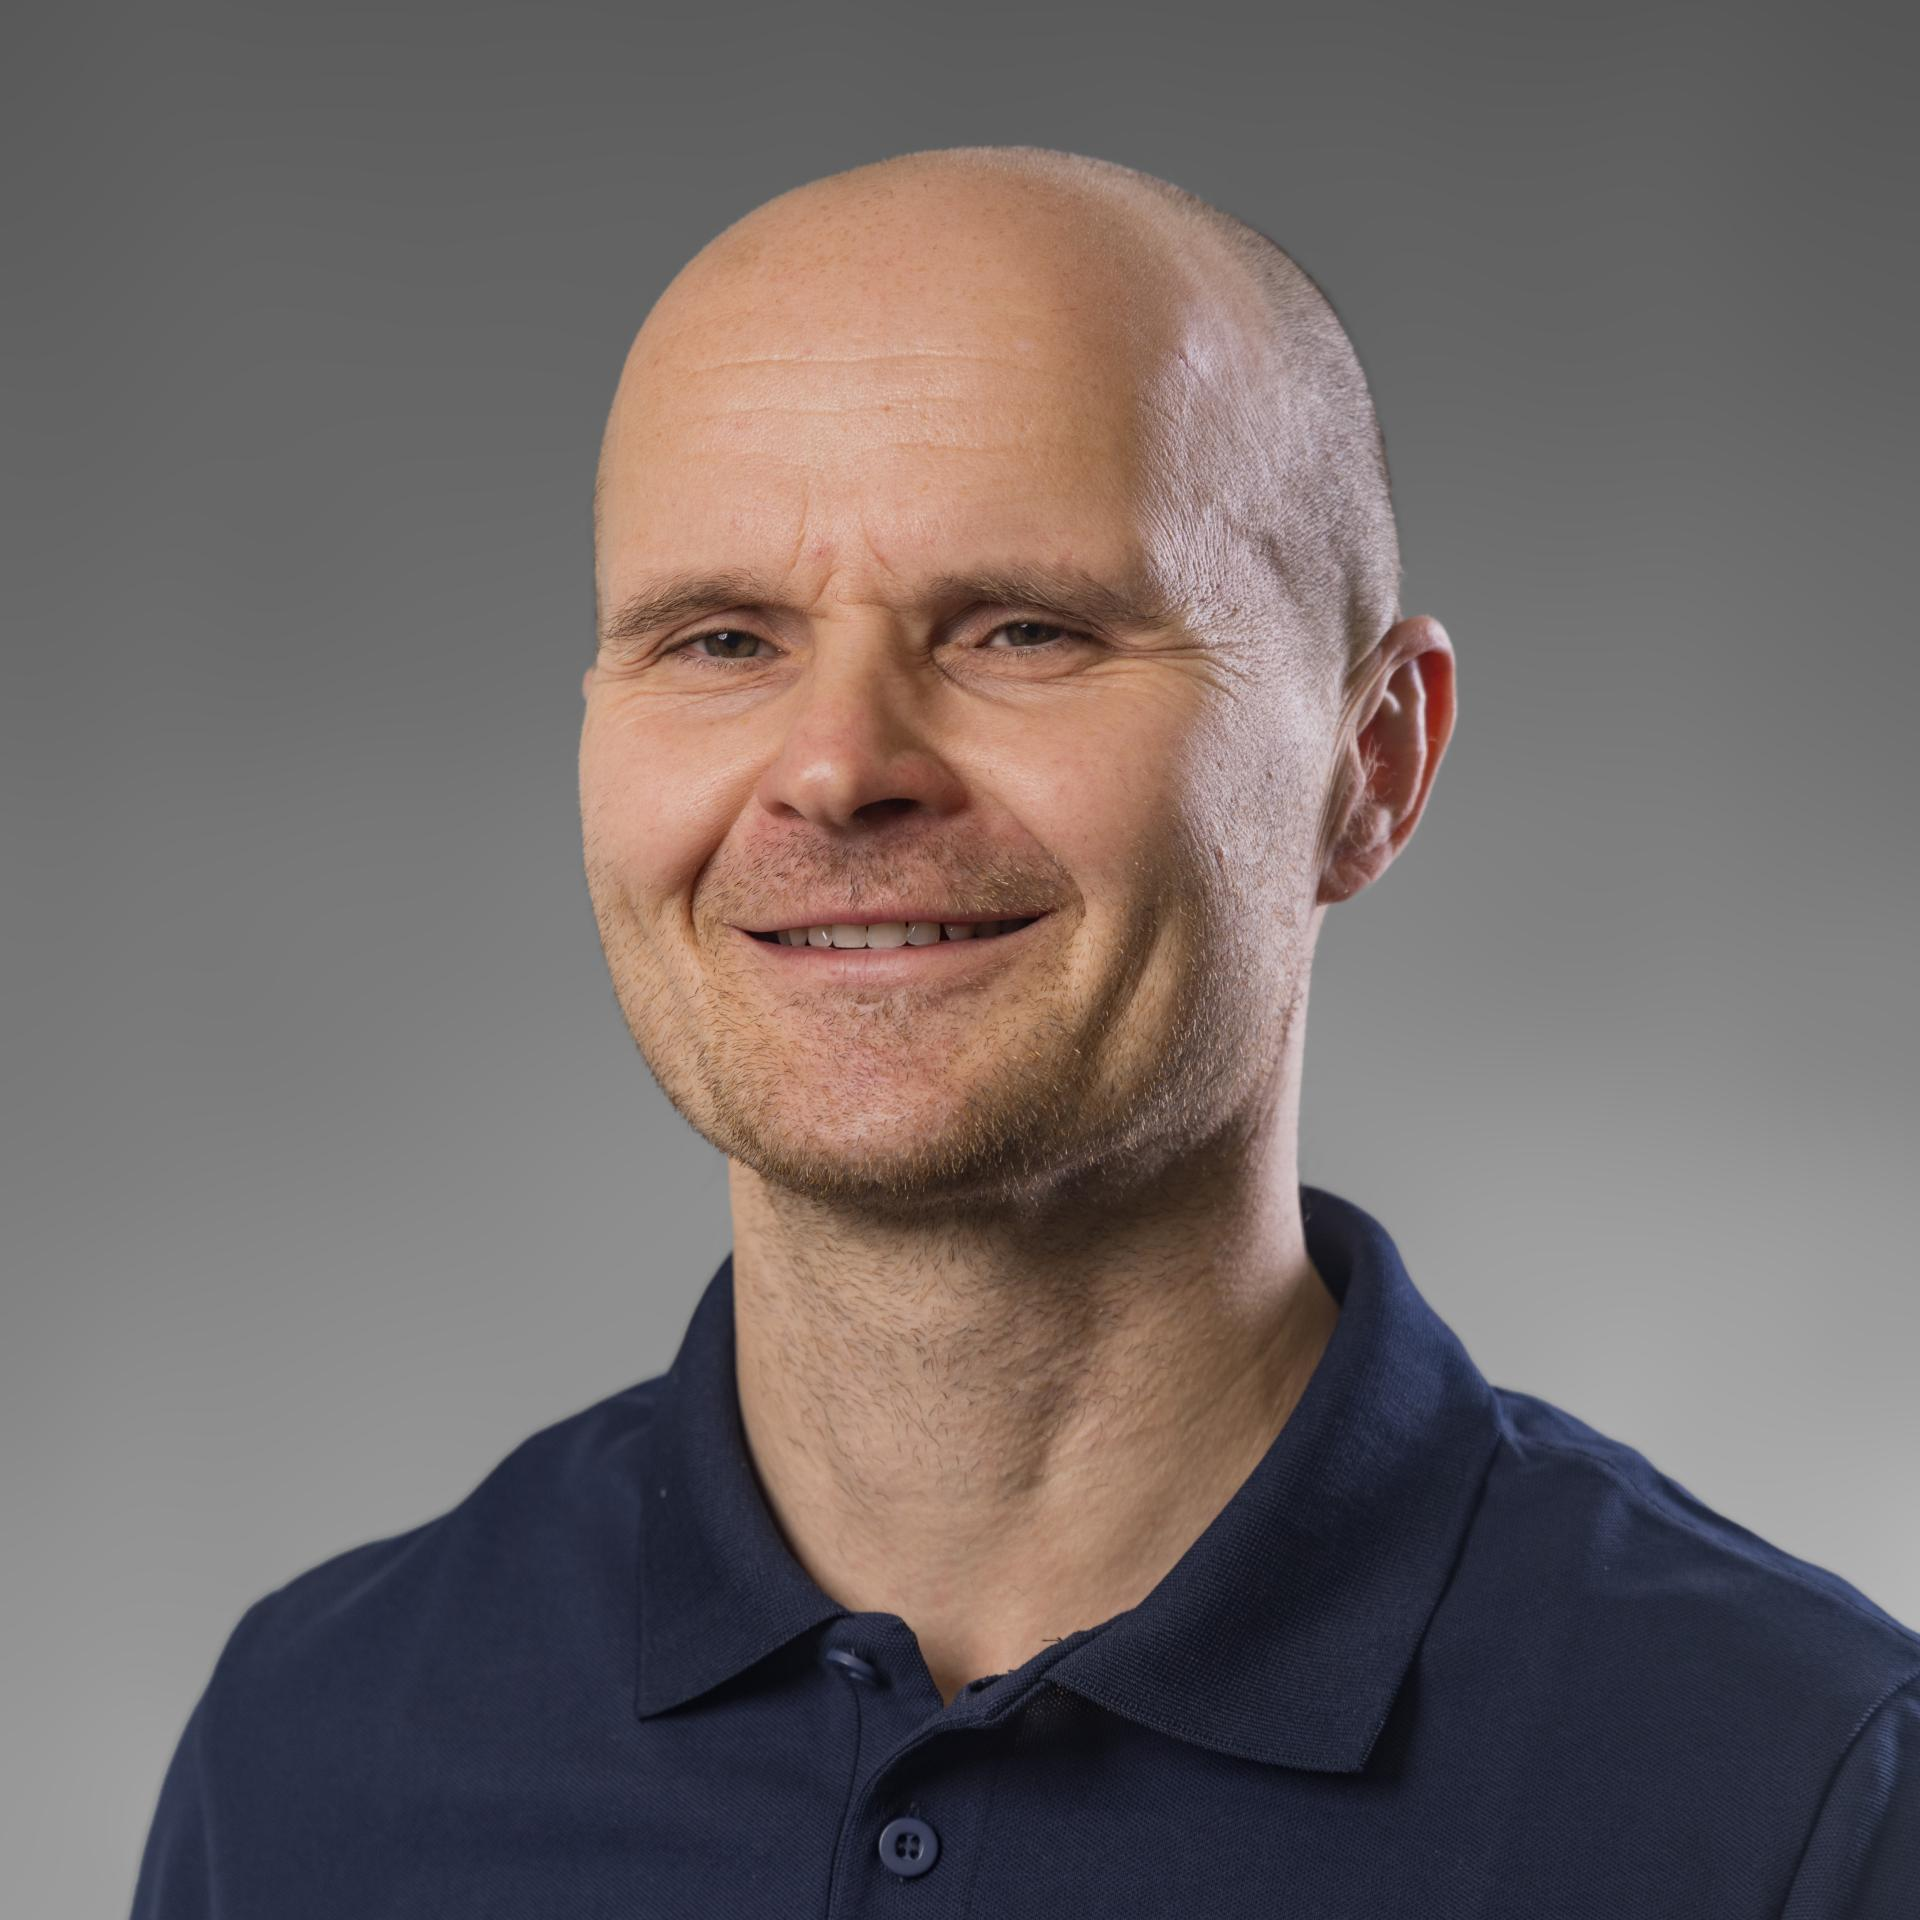
\includegraphics[width=0.8\textwidth]{Antonin-Houska-faceshot.jpg}
    \end{column}
  \end{columns}
\end{frame}

\begin{frame}
  \frametitle{Álvaro Herrera}

  \begin{columns}[T]
    \begin{column}{0.8\textwidth}
      \begin{itemize}
	\item Álvaro Herrera, EDB
	\item \href{mailto:alvherre@kurilemu.de}{\color{black}{alvherre@kurilemu.de}}
	\item Postgres contributor since 2002
	\item Working as a Postgres developer for EDB since 2012
      \end{itemize}
    \end{column}
    \begin{column}{0.2\textwidth}
      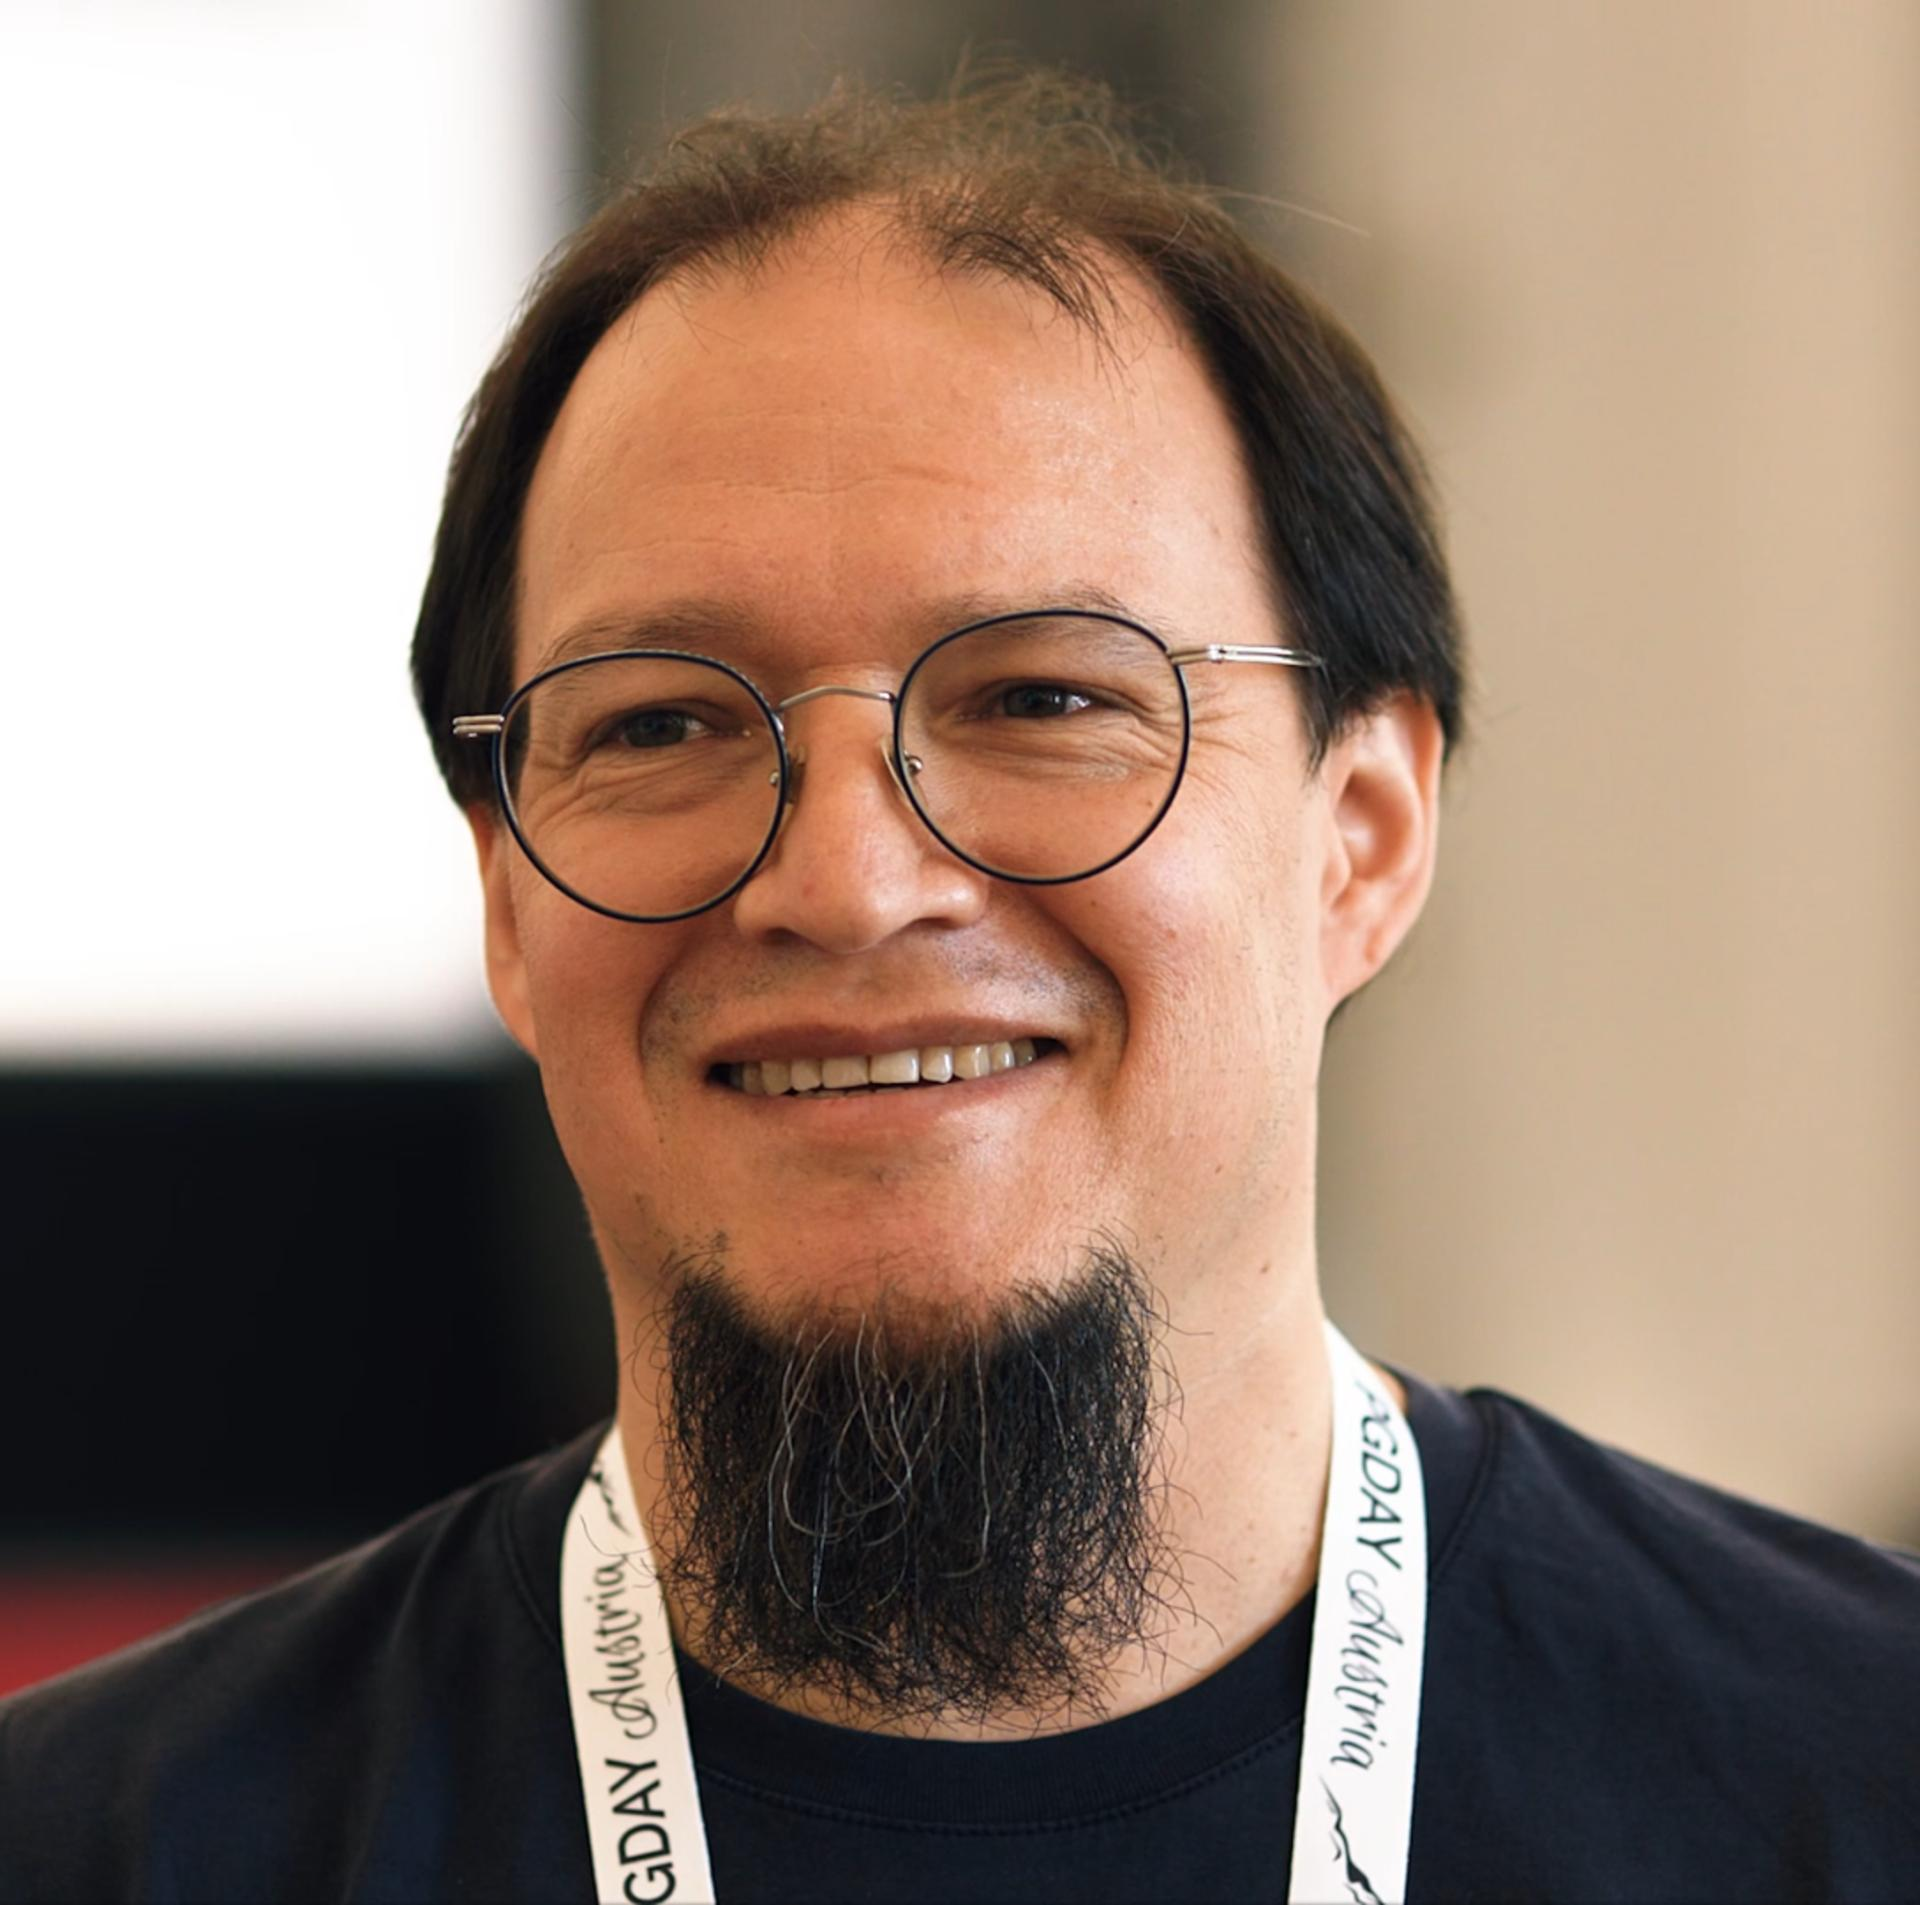
\includegraphics[width=0.8\textwidth]{alvaro-faceshot.jpg}
    \end{column}
  \end{columns}
\end{frame}

\begin{frame}
  \frametitle{Talk structure}
  \begin{enumerate}
    \item The problem: table bloat
    \item The historical solution: VACUUM and friends
    \item Third-party solutions
      \begin{itemize}
	\item \texttt{pg\_reorg}
	\item \texttt{pg\_repack}
	\item \texttt{pg\_squeeze}
      \end{itemize}
    \item Non-concurrent REPACK
    \item REPACK CONCURRENTLY
  \end{enumerate}
\end{frame}

\begin{frame}
  \frametitle{Table bloat}
  \begin{itemize}
    \item Comes from \emph{non-overwriting} MVCC implementation
    \item Non-overwriting: old versions of updated tuples are not immediately removable
    \item \emph{vacuuming}\footnote{And HOT-pruning.} takes care of them afterwards
  \end{itemize}
\end{frame}

\begin{frame}
  \frametitle{Table bloat: other databases}
  \includegraphics[width=\sizeforimages\textwidth]{images/oracle_01.png}

  An overwriting storage manager might use a ``rollback segment''
\end{frame}

\begin{frame}
  \frametitle{Table bloat: other databases}
  \includegraphics[width=\sizeforimages\textwidth]{images/oracle_02.png}

  As the table is updated, old tuples versions are moved to the rollback segment. The table doesn't need later cleanup.
\end{frame}

\begin{frame}
  \frametitle{A rollback segment?}
  \begin{itemize}
    \item requires handling of disk space for it
    \item and later cleanup
    \item notably: rollbacks are expensive
    \item<2> and is more difficult to implement
    \item<2> Postgres tried: see \texttt{zheap}
    \item<2> Not yet achieved!
  \end{itemize}
\end{frame}

\begin{frame}
  \frametitle{How 7.1 and earlier handled vacuuming}
  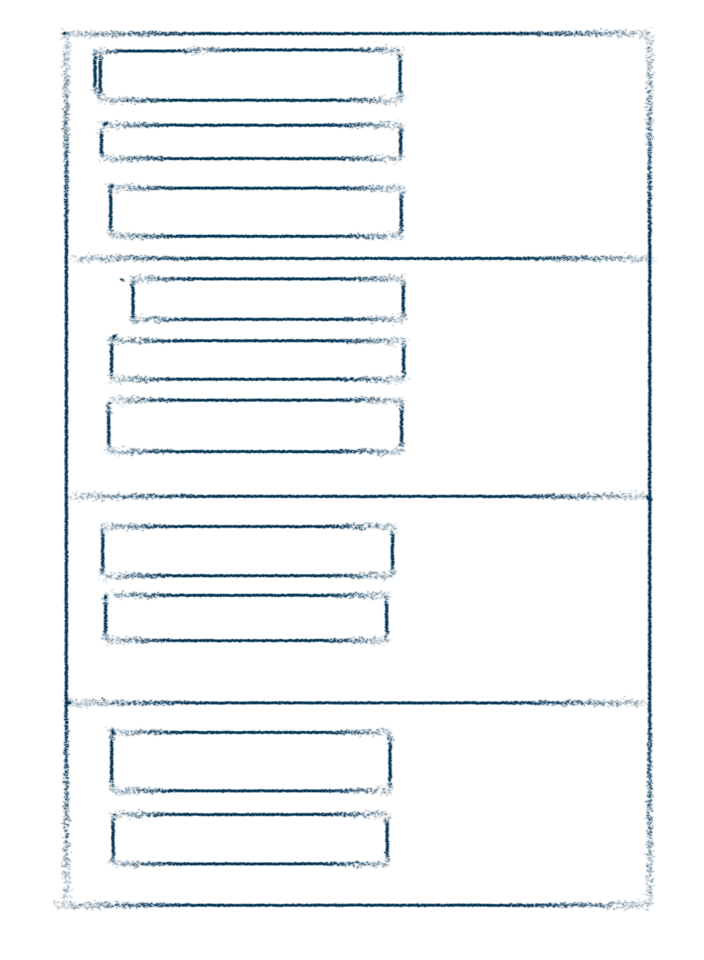
\includegraphics[height=\sizeforimages\textheight]{images/tuples.png}
\end{frame}

\begin{frame}
  \frametitle{Dead tuples}
  \begin{columns}
    \begin{column}{0.5\textwidth}
      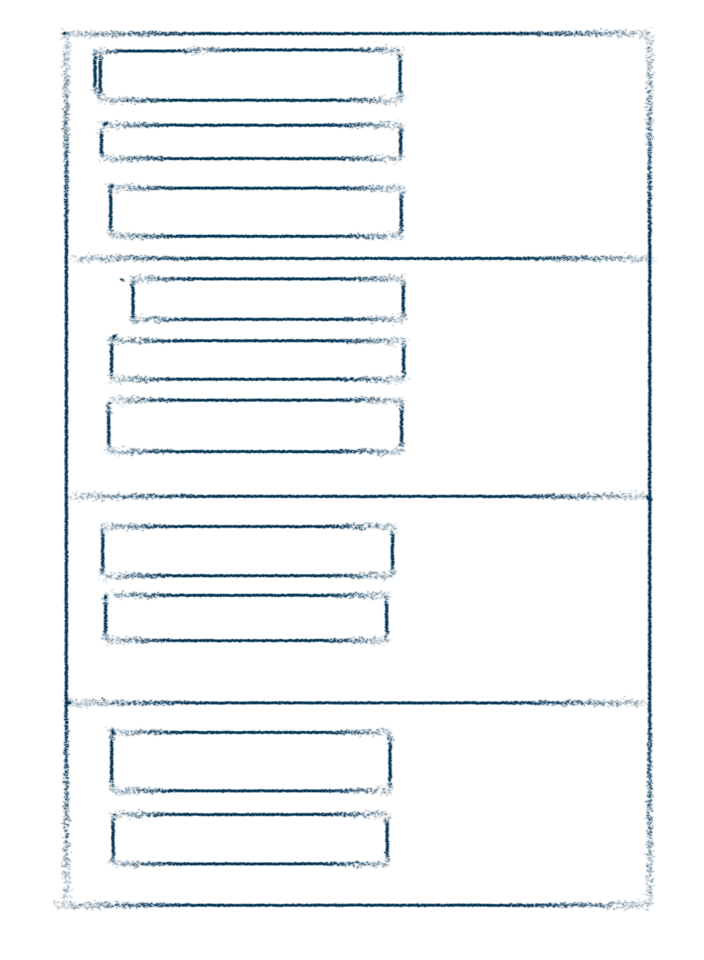
\includegraphics[height=\sizeforimages\textheight]{images/tuples.png}
    \end{column}
    \begin{column}{0.5\textwidth}
      \includegraphics[height=\sizeforimages\textheight]{images/tuples_dead.png}
    \end{column}
  \end{columns}
\end{frame}

\begin{frame}
  \frametitle{VACUUM phase 1: Dead tuples removed}
  \begin{columns}
    \begin{column}{0.33\textwidth}
      \includegraphics[height=\sizeforimages\textheight]{images/tuples_dead.png}
    \end{column}
    \begin{column}{0.33\textwidth}
      \includegraphics[height=\sizeforimages\textheight]{images/tuples_removed.png}
    \end{column}

    \begin{column}{0.33\textwidth}
      \includegraphics[height=\sizeforimages\textheight]{images/tuples_moving.png}
    \end{column}

  \end{columns}
\end{frame}

\begin{frame}
  \frametitle{VACUUM phase 2: Compact table}
  \begin{columns}
    \begin{column}{0.33\textwidth}
      \includegraphics[height=\sizeforimages\textheight]{images/tuples_moving.png}
    \end{column}
    \begin{column}{0.33\textwidth}
      \includegraphics[height=\sizeforimages\textheight]{images/tuples_compacted.png}
    \end{column}
  \end{columns}
\end{frame}

\begin{frame}
  \frametitle{``Lazy'' vacuum?}
  \begin{itemize}
    \item But this required ``access exclusive'' lock on the table
    \item {\linksize \href{https://git.postgresql.org/cgit/postgresql.git/commit/?id=4046e58c2478cfcdd4334e2c282b5a42f047ea0b}
      {Commit 4046e58c2478: \faExternalLink \\
      Initial implementation of concurrent VACUUM. \\
      Tom Lane \\
      Fri Jul 13 2001, Postgres 7.2}}
    \item Doesn't require access exclusive lock anymore
    \item Operation can continue
    \item Disadvantage: surviving tuples cannot be moved across pages
    \item Old-style vacuum is renamed \texttt{VACUUM FULL}
  \end{itemize}
\end{frame}



\begin{frame}
  \frametitle{The problem: table bloat}
  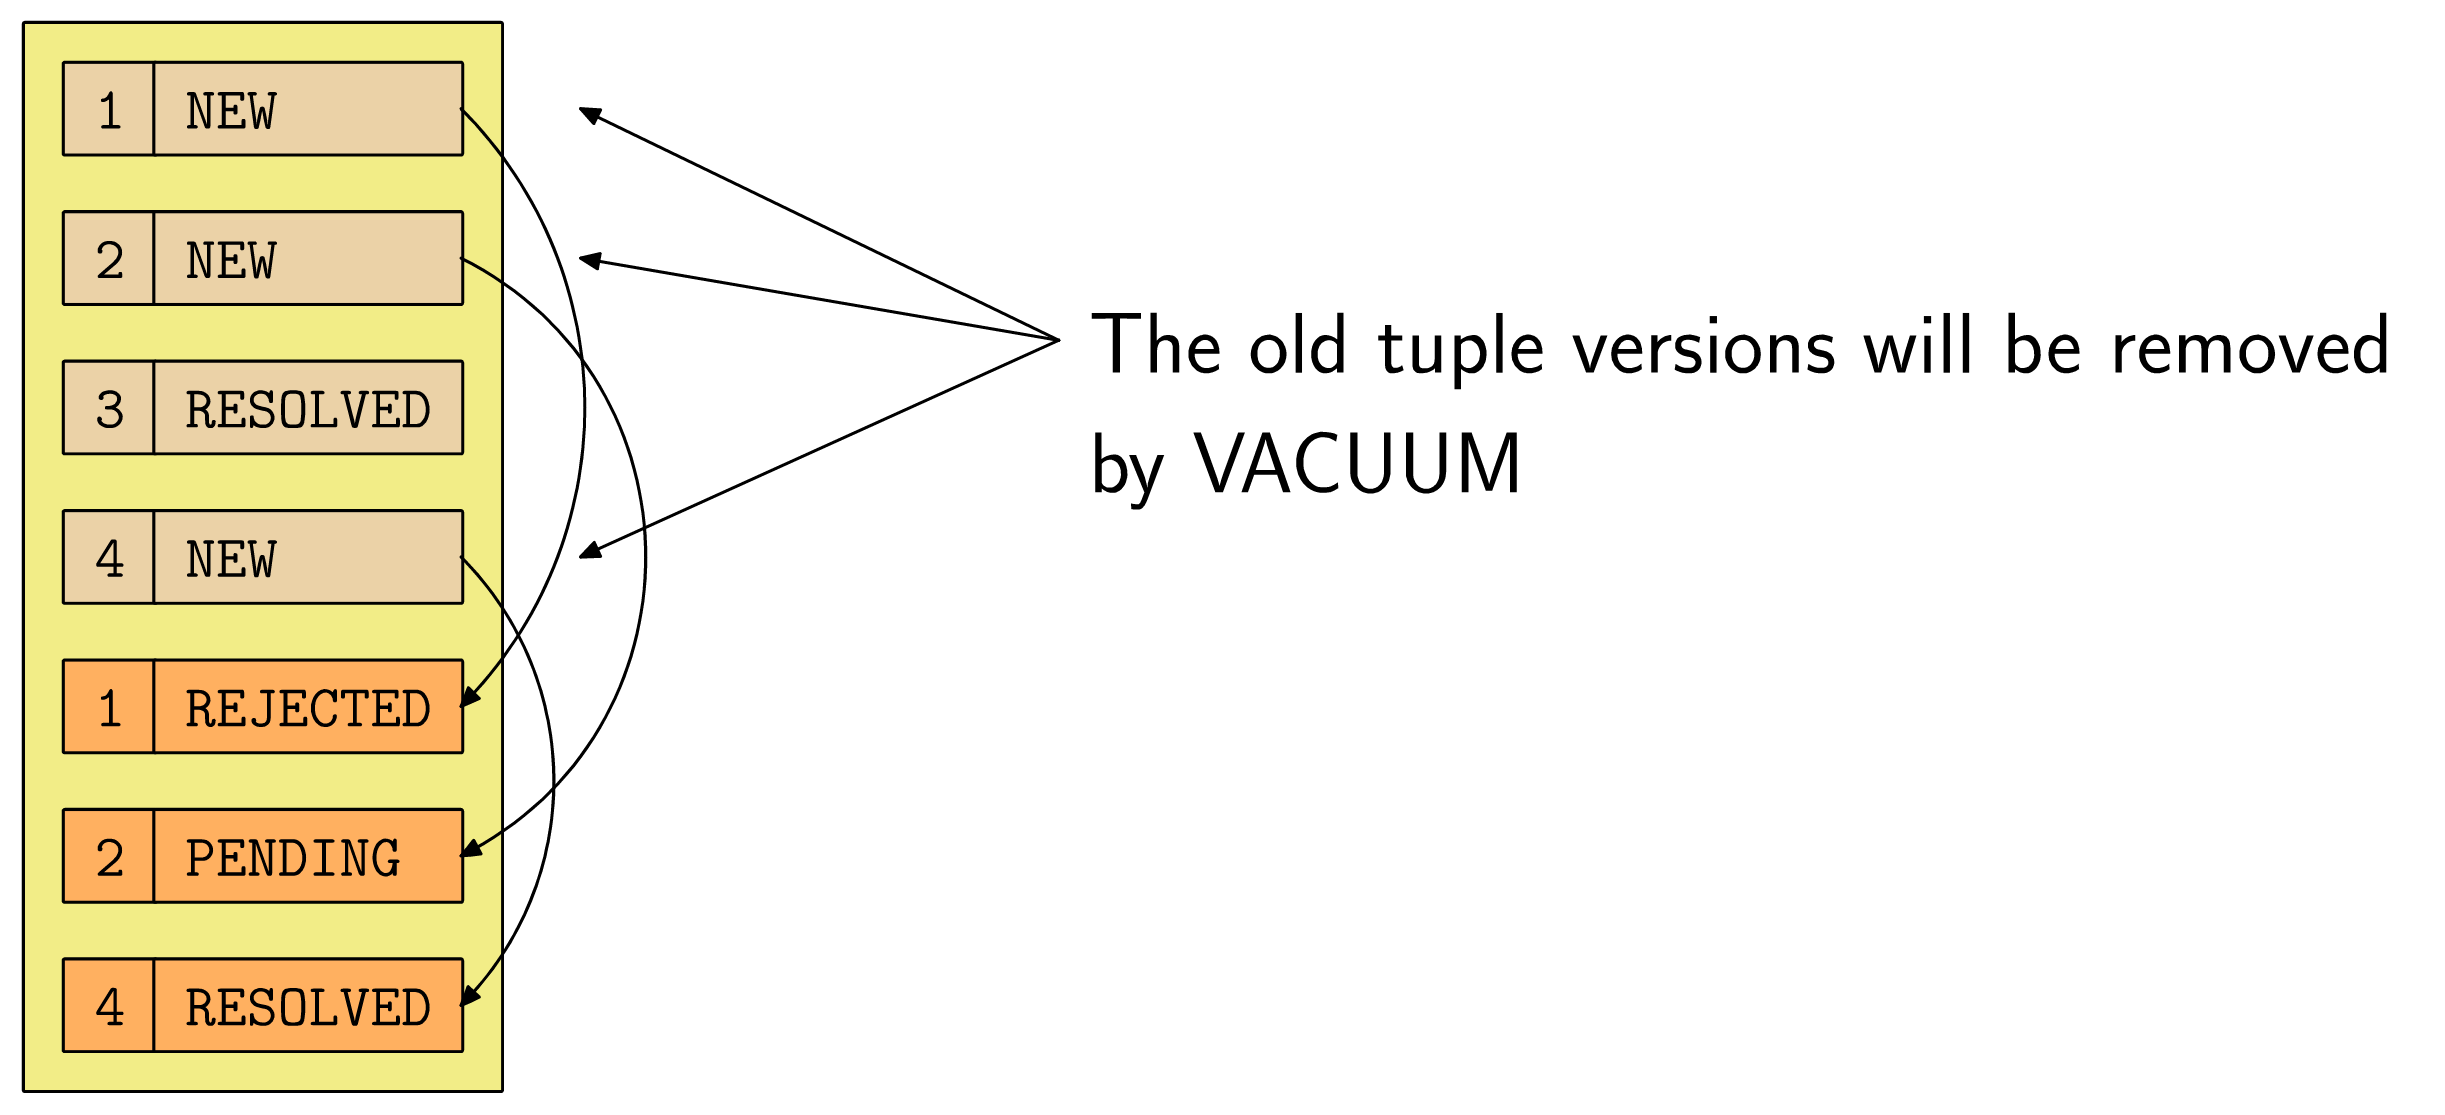
\includegraphics[height=\sizeforimages\textheight]{images/bloat_01.png}
\end{frame}

\begin{frame}
  \frametitle{The problem: table bloat}
  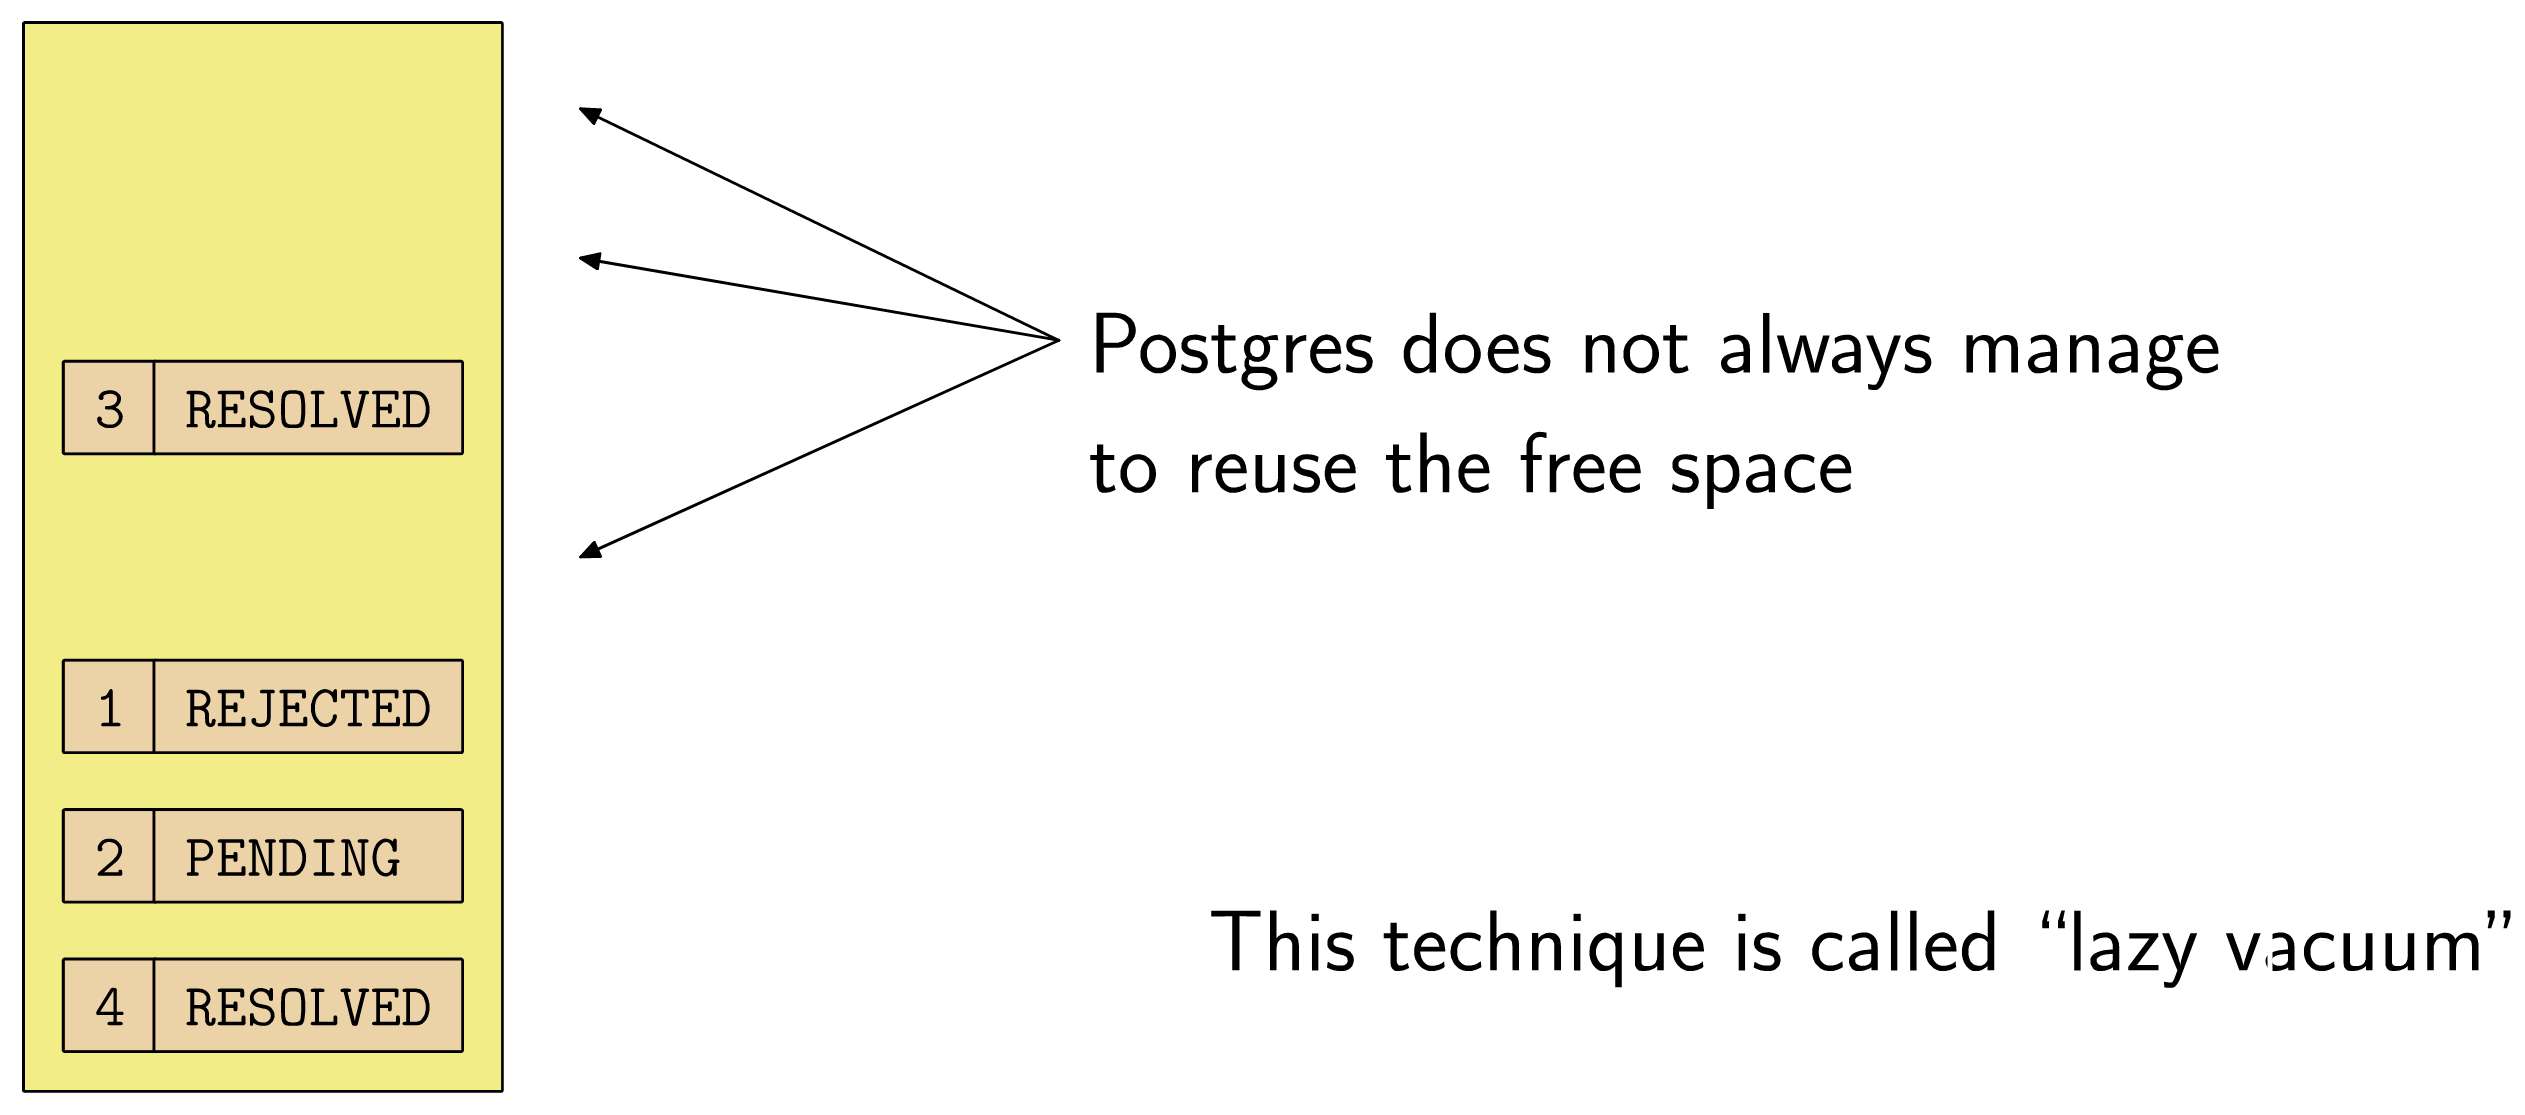
\includegraphics[height=\sizeforimages\textheight]{images/bloat_02.png}
\end{frame}

\begin{frame}
  \frametitle{A faster VACUUM FULL?}
  \begin{itemize}

    \item Yes! \emph{``Let's use \texttt{CLUSTER},'' someone said}
    \item {\linksize \href{https://git.postgresql.org/cgit/postgresql.git/commit/?id=946cf229e89fda779161d707f3ba1f4d3cd024a1}
      {Commit 946cf229e89f: \faExternalLink \\
      Support rewritten-based full vacuum as VACUUM FULL. Traditional VACUUM FULL was renamed to VACUUM FULL INPLACE. \\
      Itagaki Takahiro \\
      Wed Jan 6 2010, Postgres 9.0}}

    \item In 2010 (Postgres 9.0), VACUUM FULL was changed to use the CLUSTER code
      % commit 946cf229e89fda779161d707f3ba1f4d3cd024a1
    \item How does this work?
  \end{itemize}
\end{frame}

\begin{frame}
  \frametitle{\texttt{CLUSTER}-based \texttt{VACUUM FULL}}
  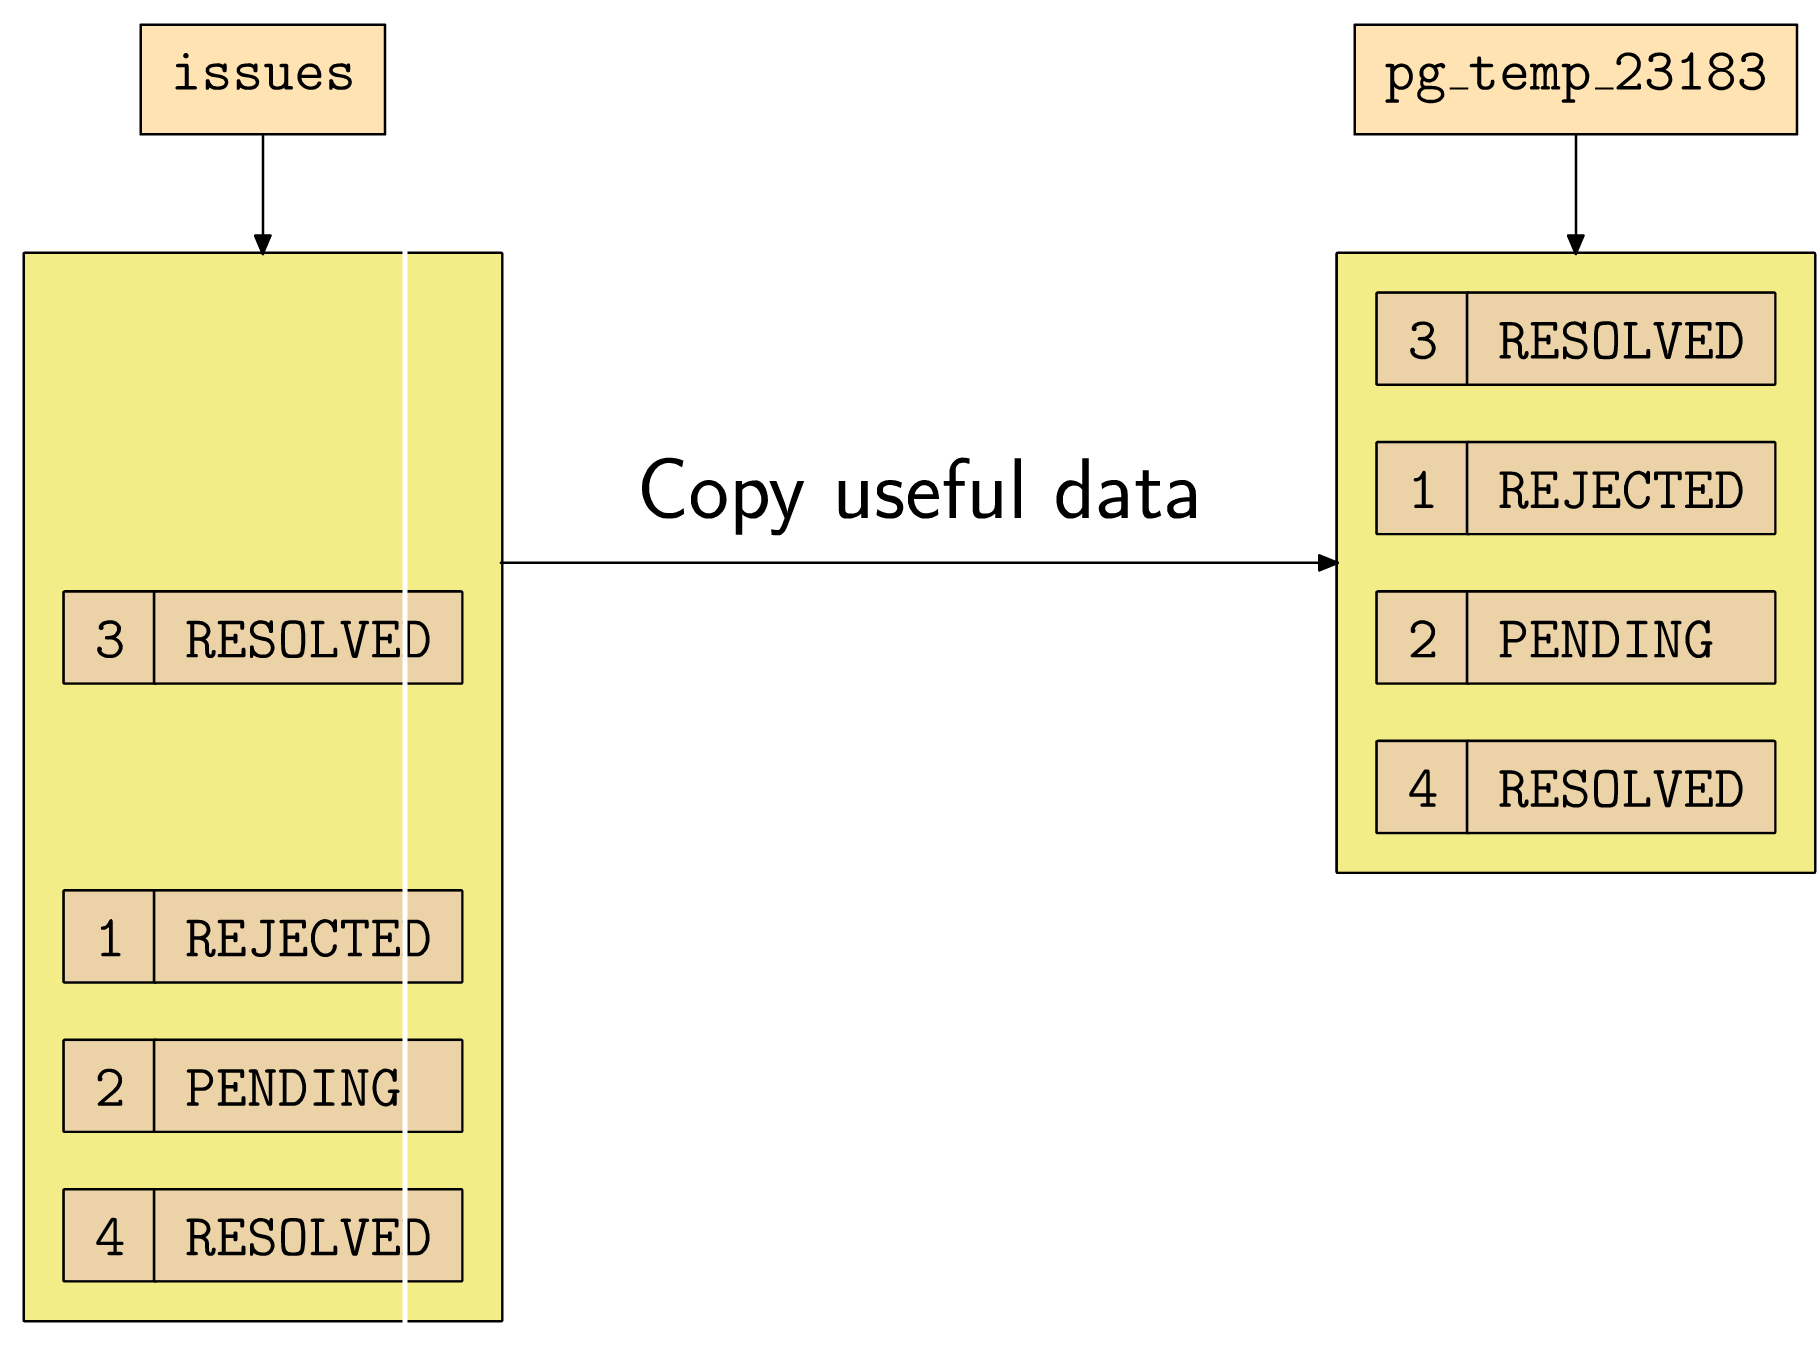
\includegraphics[height=\sizeforimages\textheight]{images/vacuum_full_01.png}
\end{frame}

\begin{frame}
  \frametitle{\texttt{CLUSTER}-based \texttt{VACUUM FULL}}
  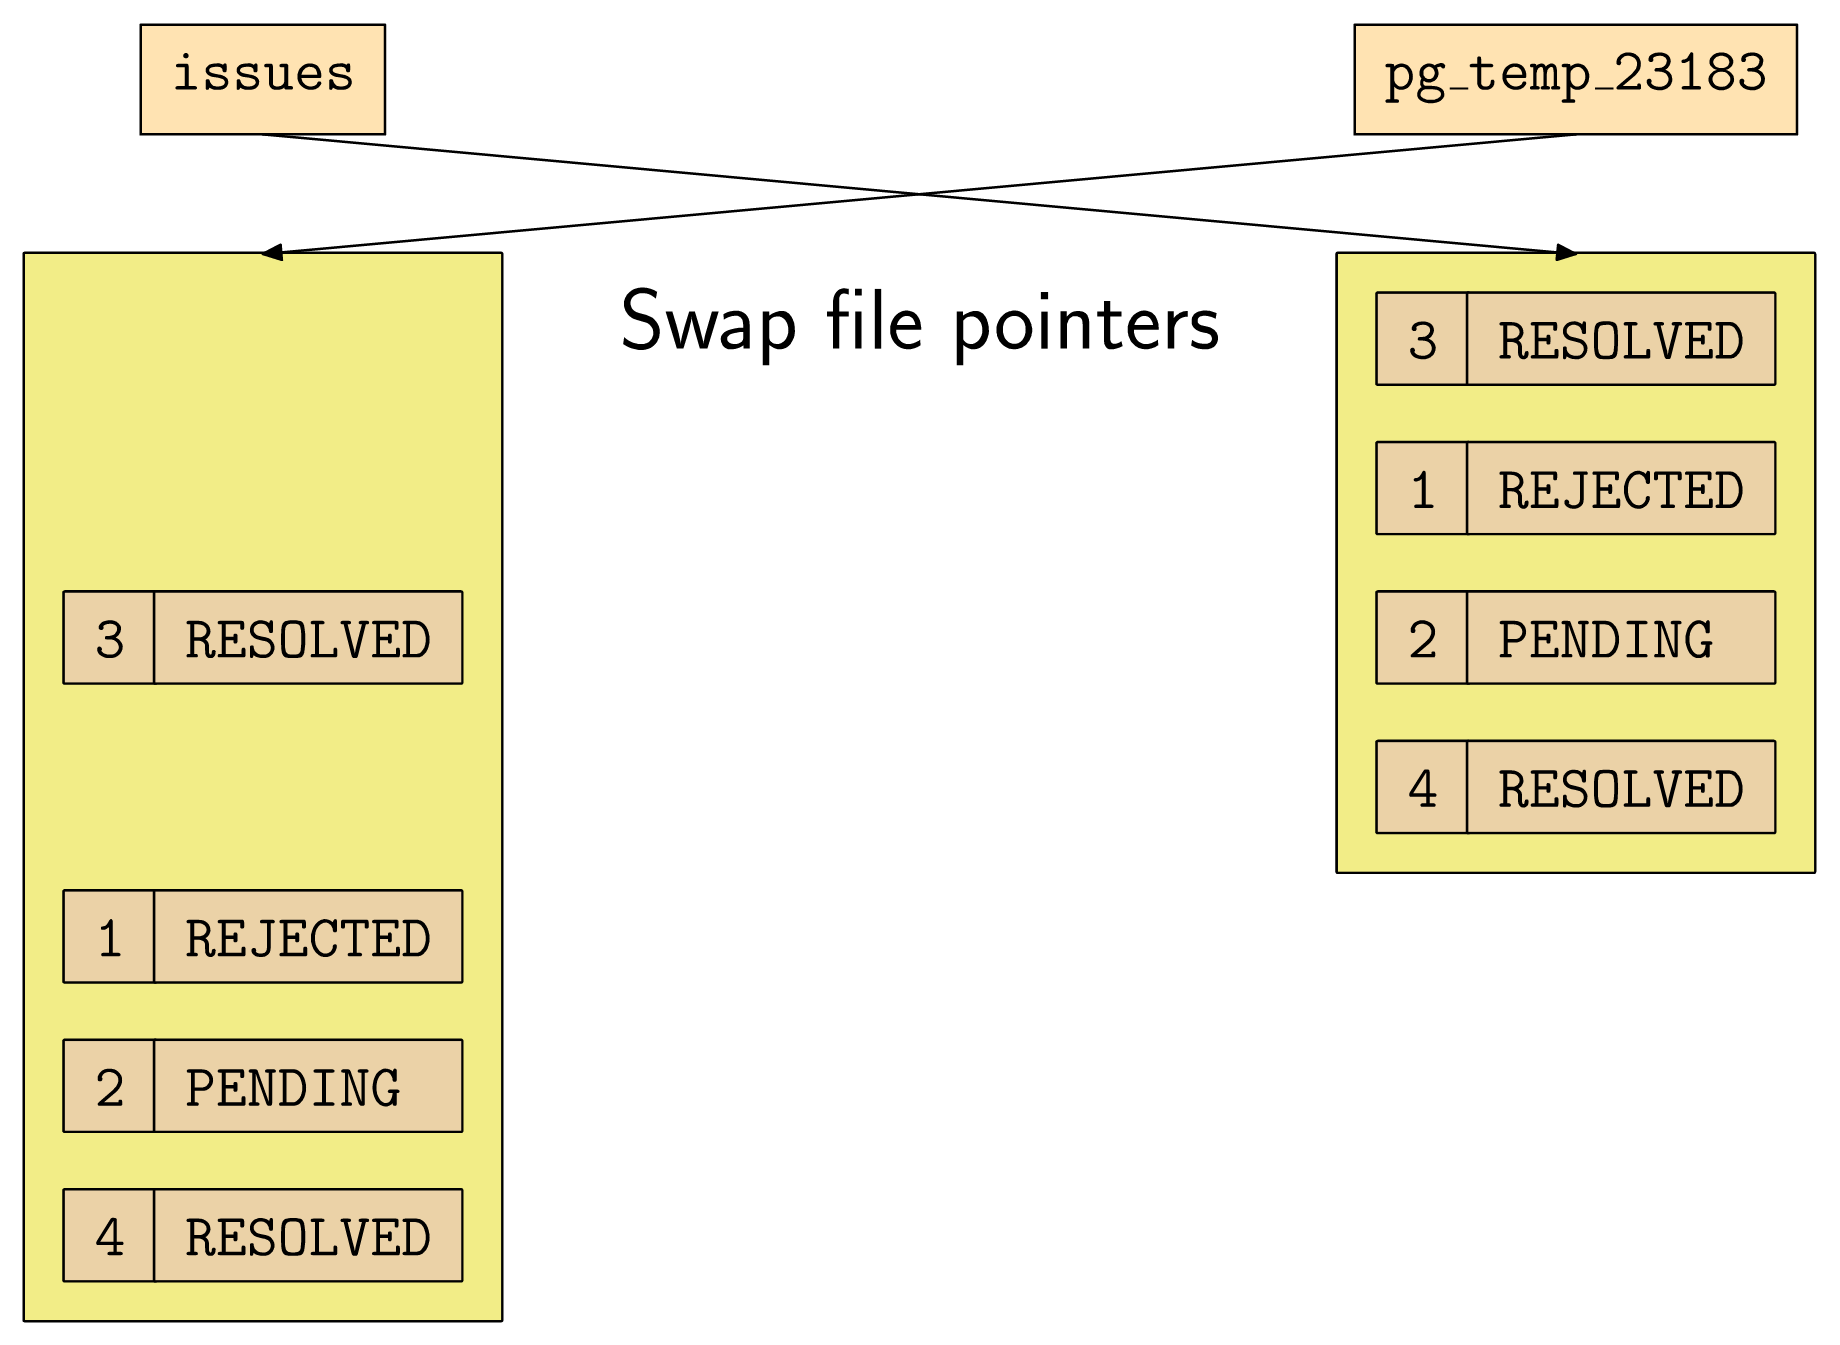
\includegraphics[height=\sizeforimages\textheight]{images/vacuum_full_02.png}
\end{frame}

% \begin{frame}
%   \frametitle{Exclusive lock is needed}
%   \begin{center}
%     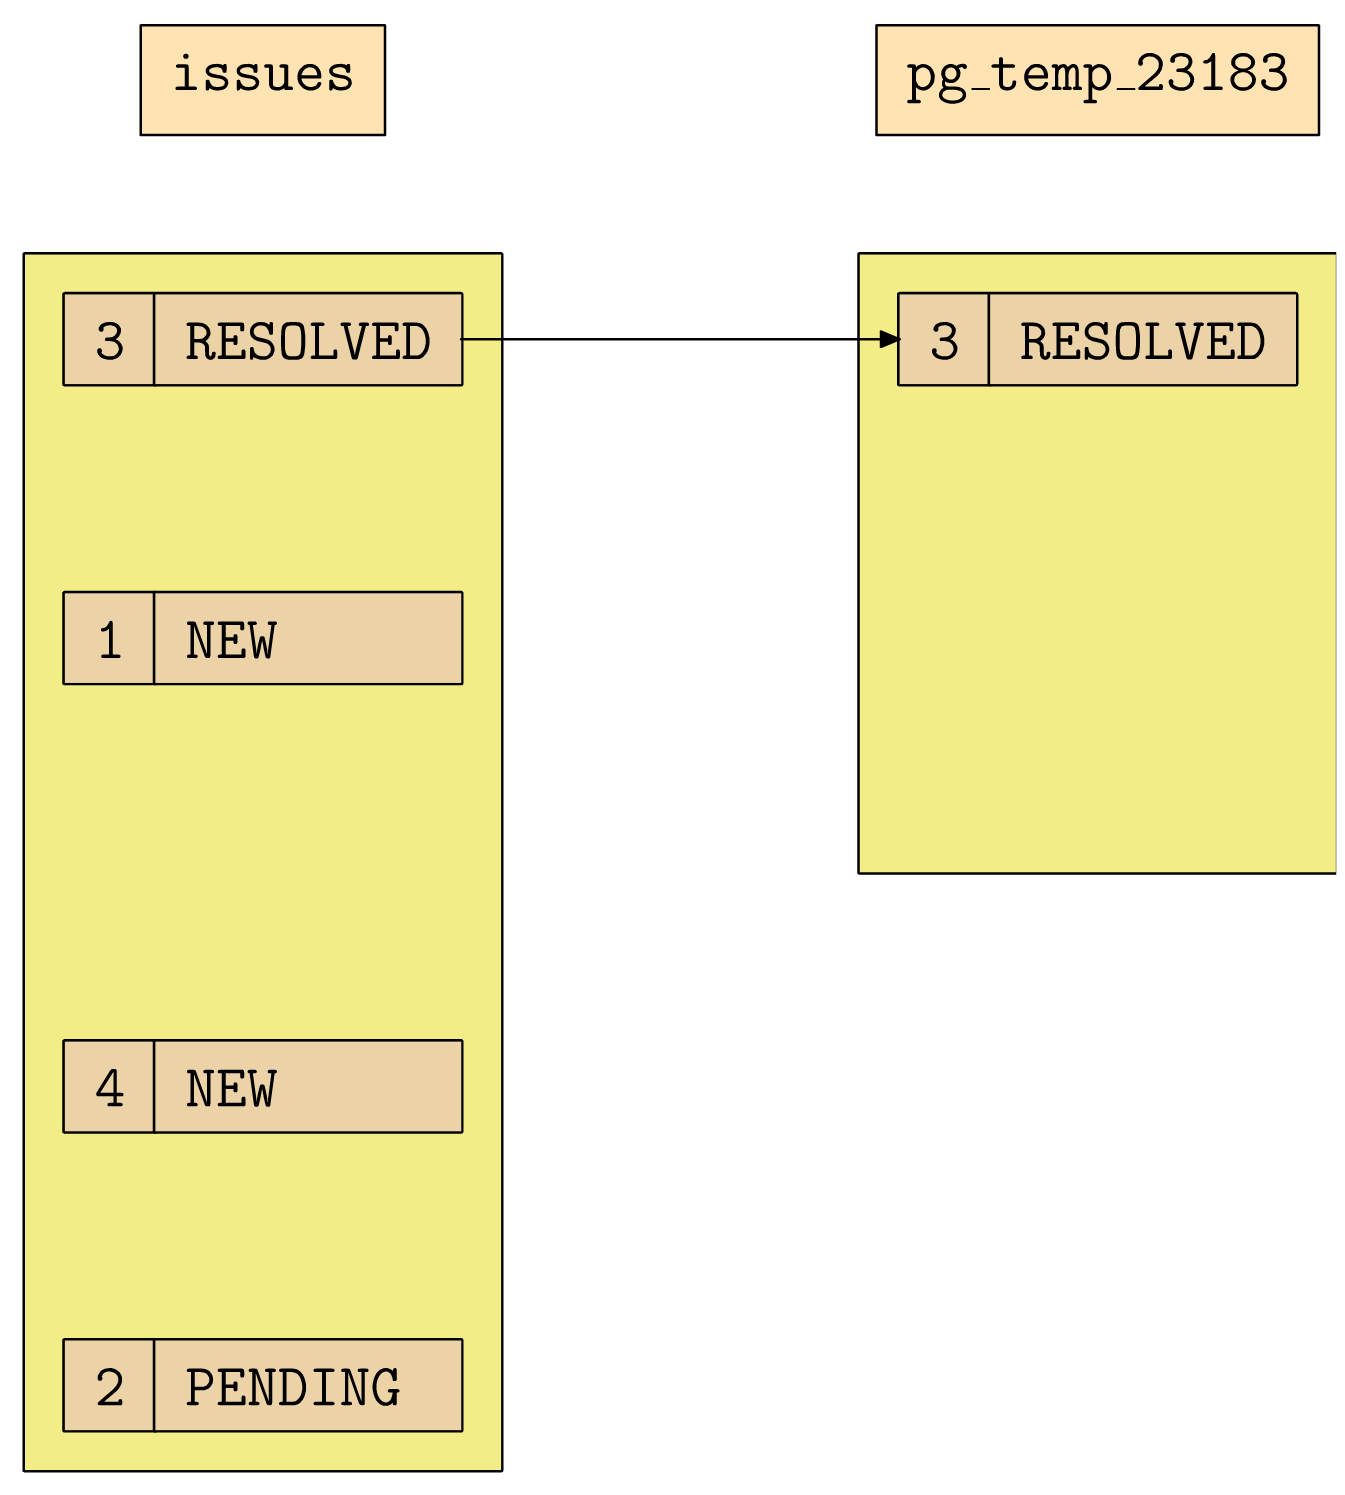
\includegraphics[height=\sizeforimages\textheight]{images/exclusive_lock_needed_01.png}
%   \end{center}
% \end{frame}
% 
% \begin{frame}
%   \frametitle{Exclusive lock is needed}
%   \begin{center}
%     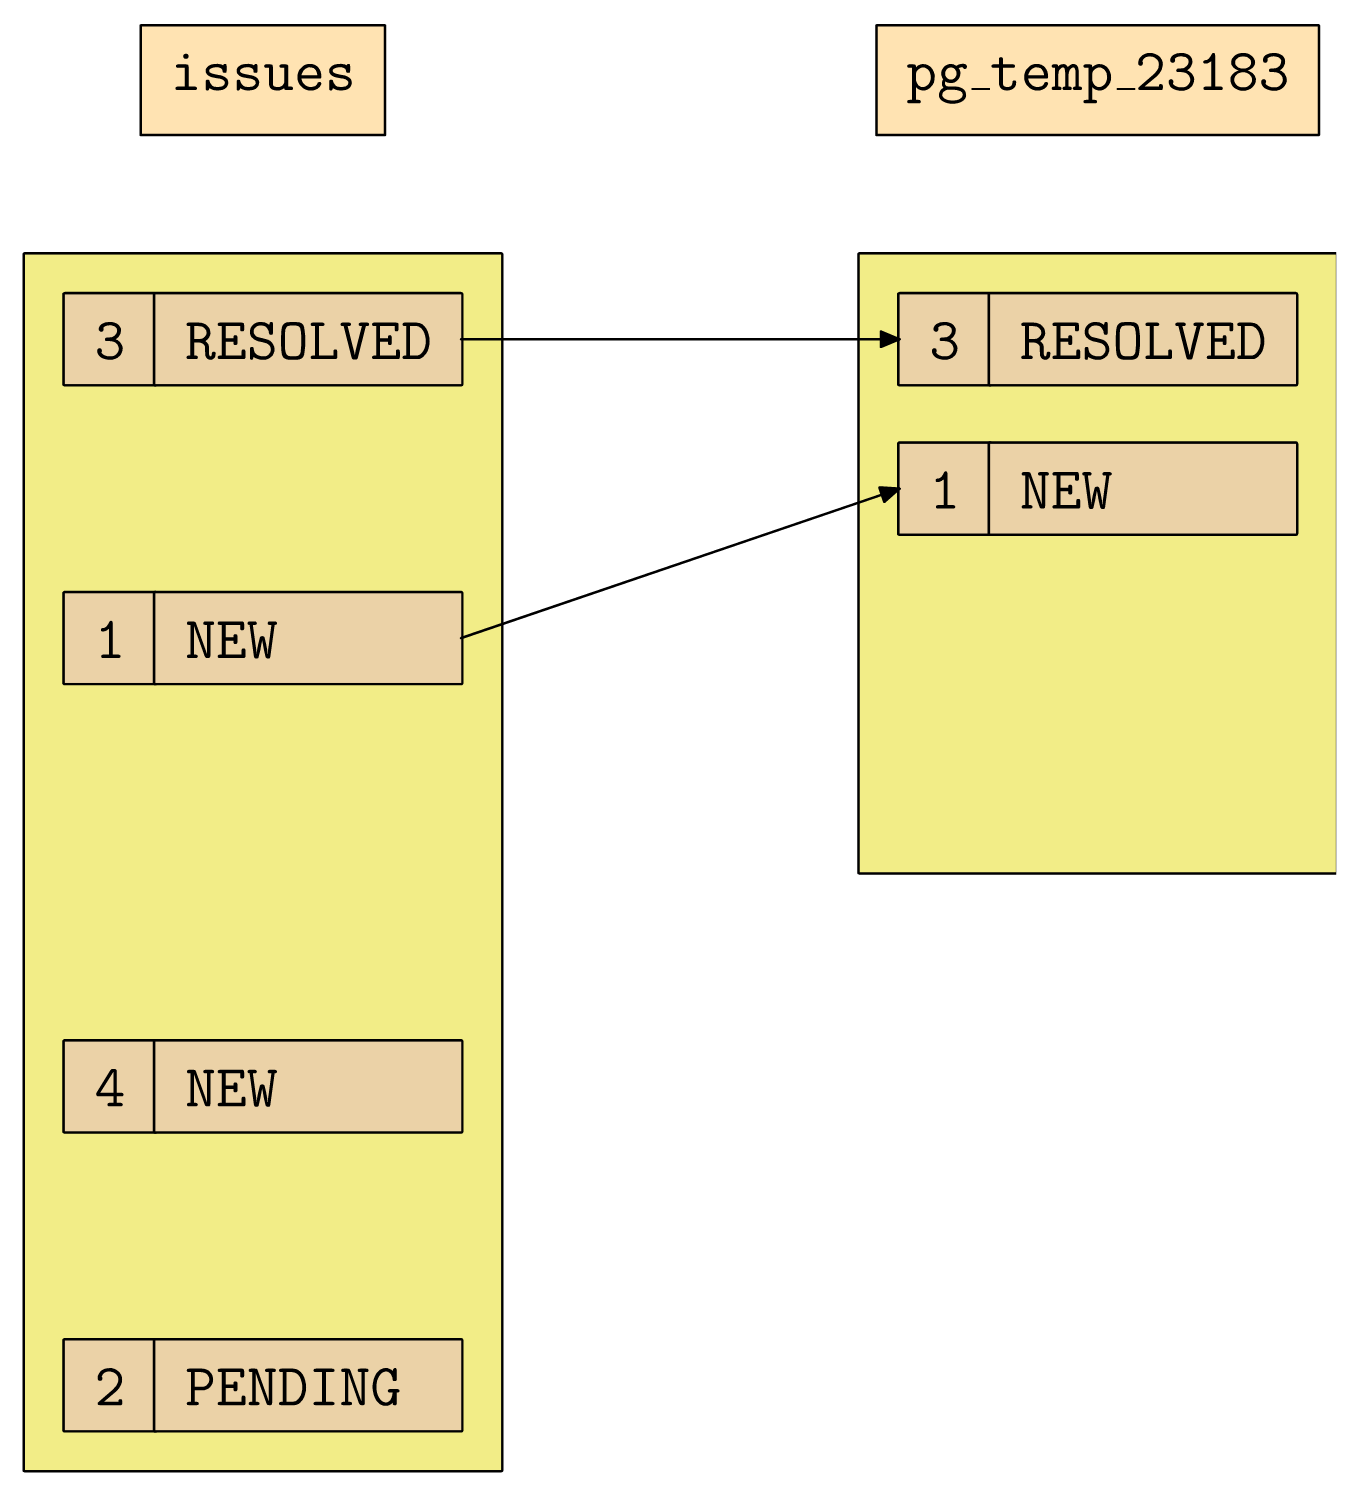
\includegraphics[height=\sizeforimages\textheight]{images/exclusive_lock_needed_02.png}
%   \end{center}
% \end{frame}
% 
% \begin{frame}
%   \frametitle{Exclusive lock is needed}
%   \begin{center}
%     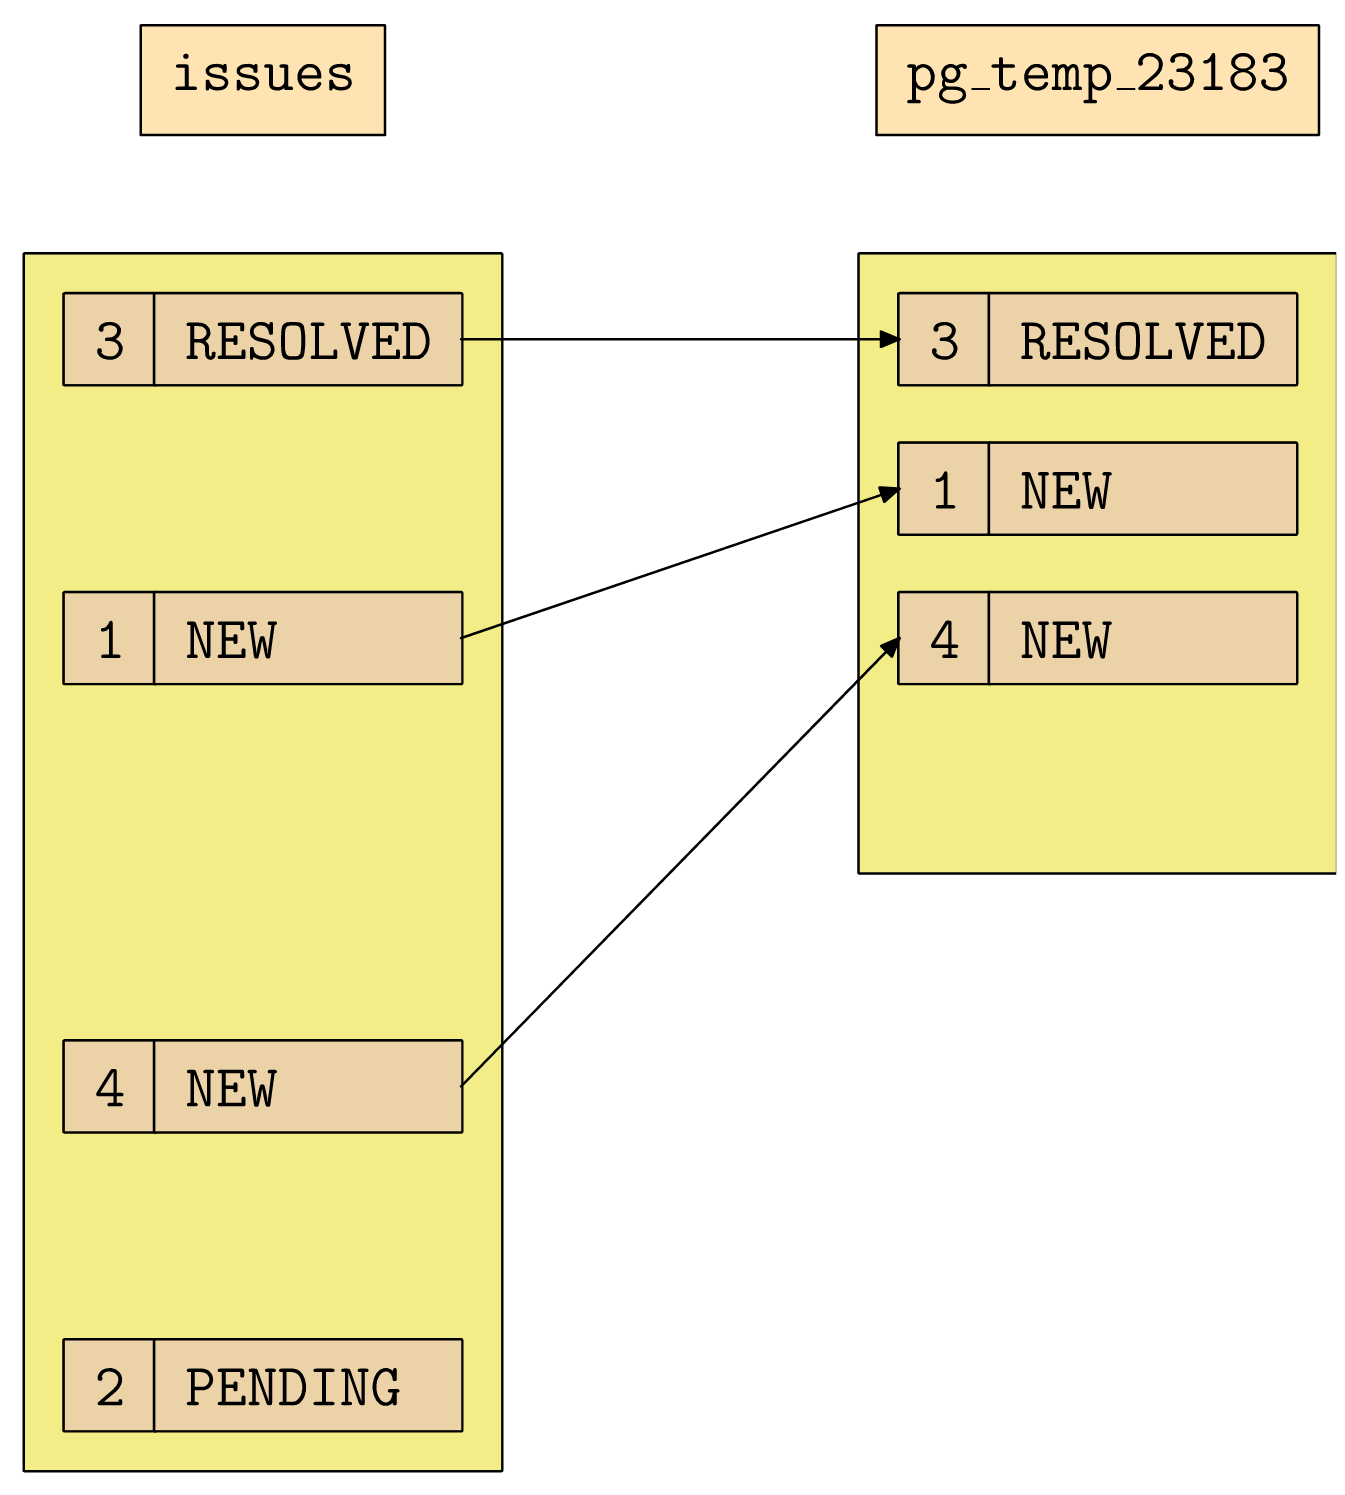
\includegraphics[height=\sizeforimages\textheight]{images/exclusive_lock_needed_03.png}
%   \end{center}
% \end{frame}
% 
% \begin{frame}
%   \frametitle{Exclusive lock is needed}
%   \begin{center}
%     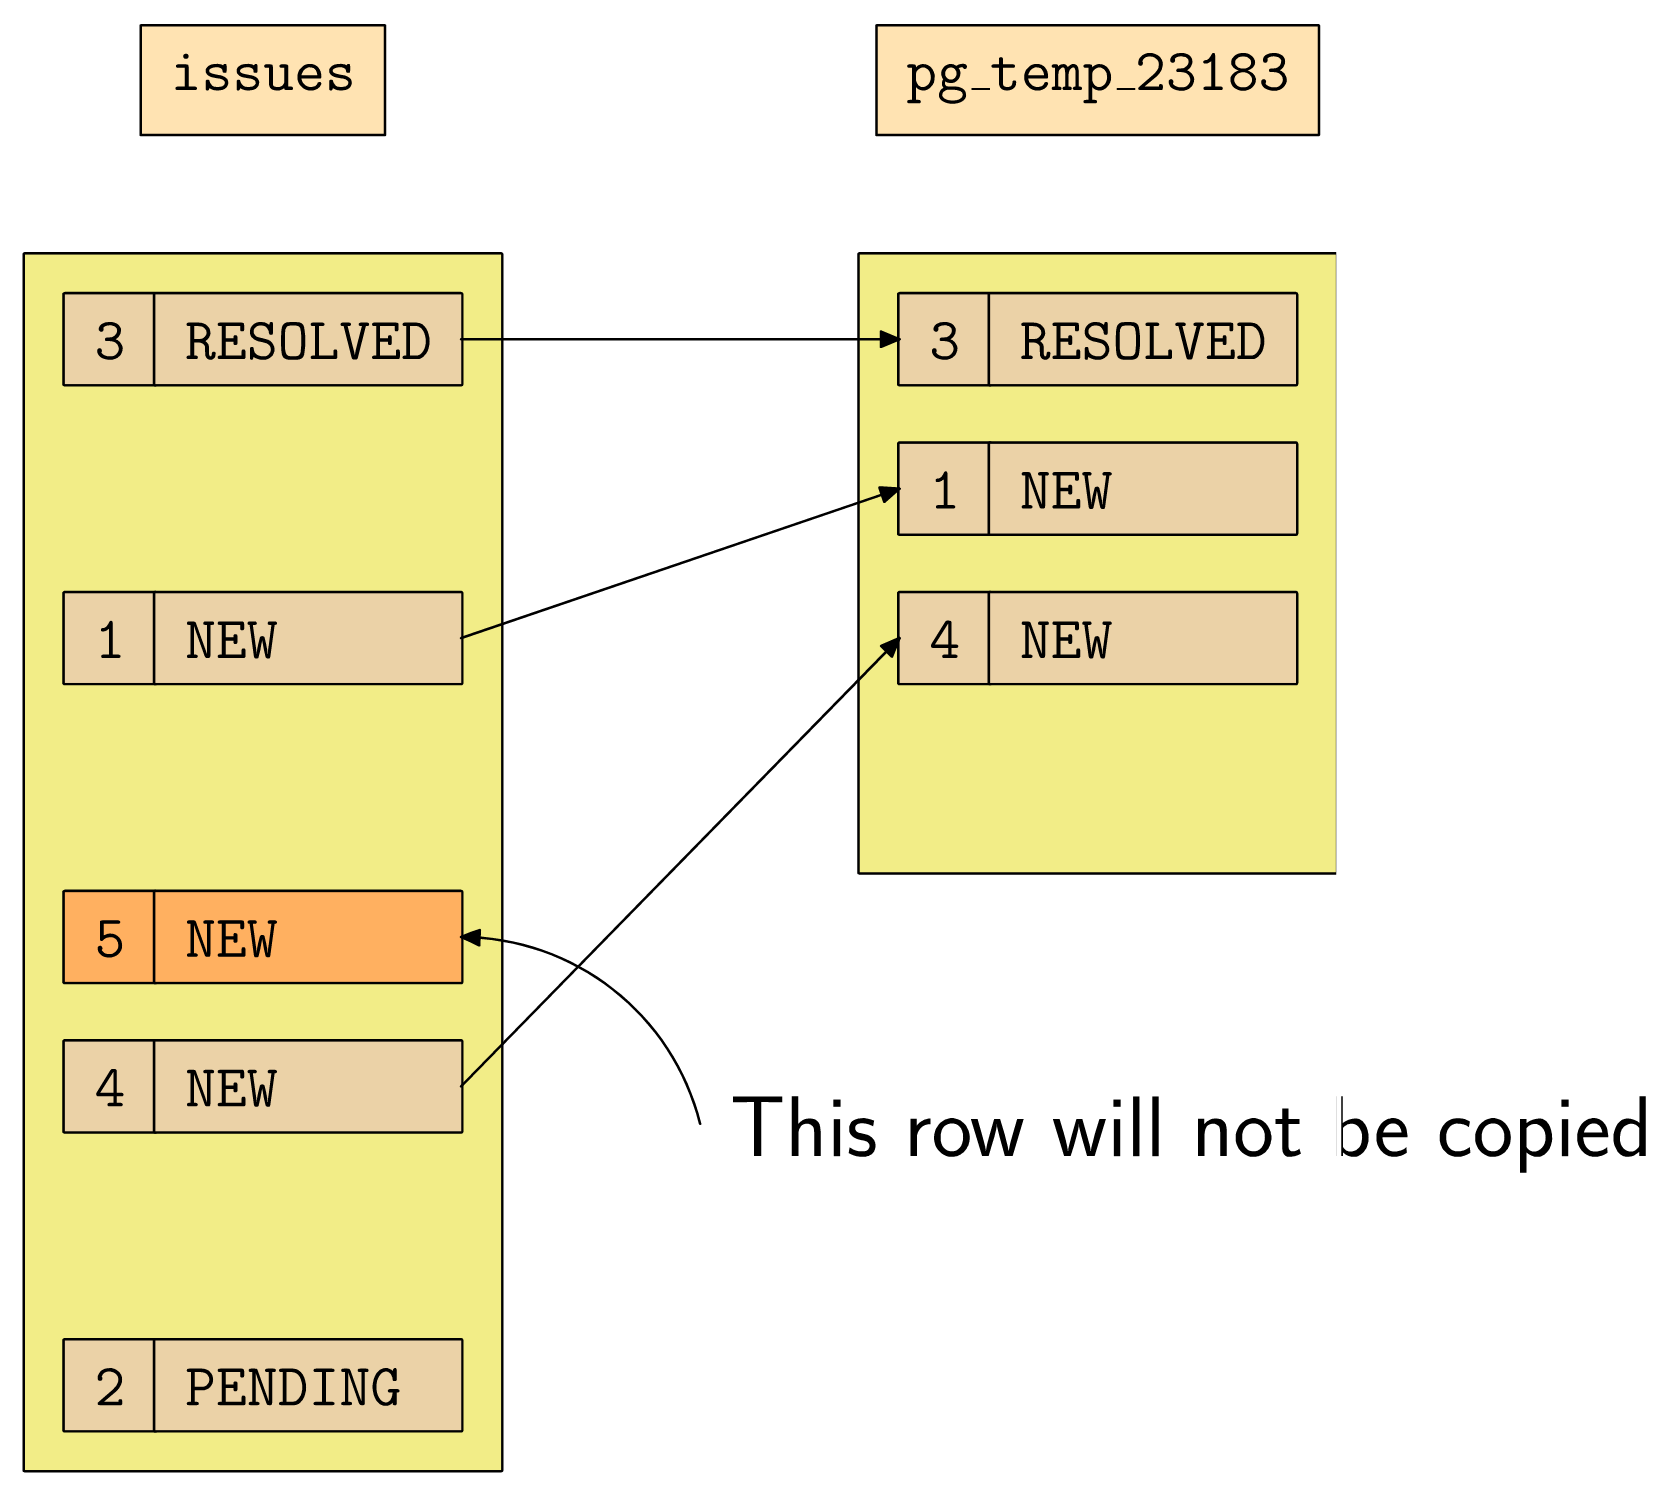
\includegraphics[height=\sizeforimages\textheight]{images/exclusive_lock_needed_04.png}
%   \end{center}
% \end{frame}

\begin{frame}
  \frametitle{\texttt{VACUUM FULL INPLACE} removed}
  \begin{itemize}
    \item {\linksize \href{https://git.postgresql.org/cgit/postgresql.git/commit/?id=0a469c87692d15a22eaa69d4b3a43dd8e278dd64}
      {Commit 0a469c87692d: \faExternalLink \\
      Remove old-style VACUUM FULL (which was known for a little while as
      VACUUM FULL INPLACE), along with a boatload of subsidiary code and complexity.
      Per discussion, the use case for this method of vacuuming is no longer large
      enough to justify maintaining it; not to mention that we don't wish to invest
      the work that would be needed to make it play nicely with Hot Standby. \\
      Tom Lane \\
      Mon Feb 8 2010, Postgres 9.0}}
  \end{itemize}
\end{frame}

\begin{frame}
  \frametitle{\texttt{pg\_reorg}}
  \begin{itemize}
    \item Created in 2008 by NTT
    \item \href{https://ossc-db.github.io/pg_reorg/pg_reorg.html}{\texttt{https://ossc-db.github.io/pg\_reorg/}}
      \begin{quote}
	``The module is developed to be a better alternative of CLUSTER and VACUUM FULL.''
      \end{quote}
    \item Featured in Depesz's blog in 2011: \href{https://www.depesz.com/2011/07/06/bloat-happens/}{Bloat Happens}
      \begin{quote}
	``All in all – it's a great tool, which does amazing job.''
      \end{quote}
    \item Last release was 1.1.9 in 2013
    \item Pronounced dead in 2020
  \end{itemize}
\end{frame}

\begin{frame}
  \frametitle{\texttt{pg\_repack}}
  \begin{itemize}
    \item Forked from \texttt{pg\_reorg} in 2012
    \item Implemented in two parts:
      \begin{itemize}
	\item A few server-side SQL and C functions
	\item Workflow controlled by a client application
      \end{itemize}
  \end{itemize}
\end{frame}

\begin{frame}
  \frametitle{\texttt{pg\_repack}}
  \begin{center}
    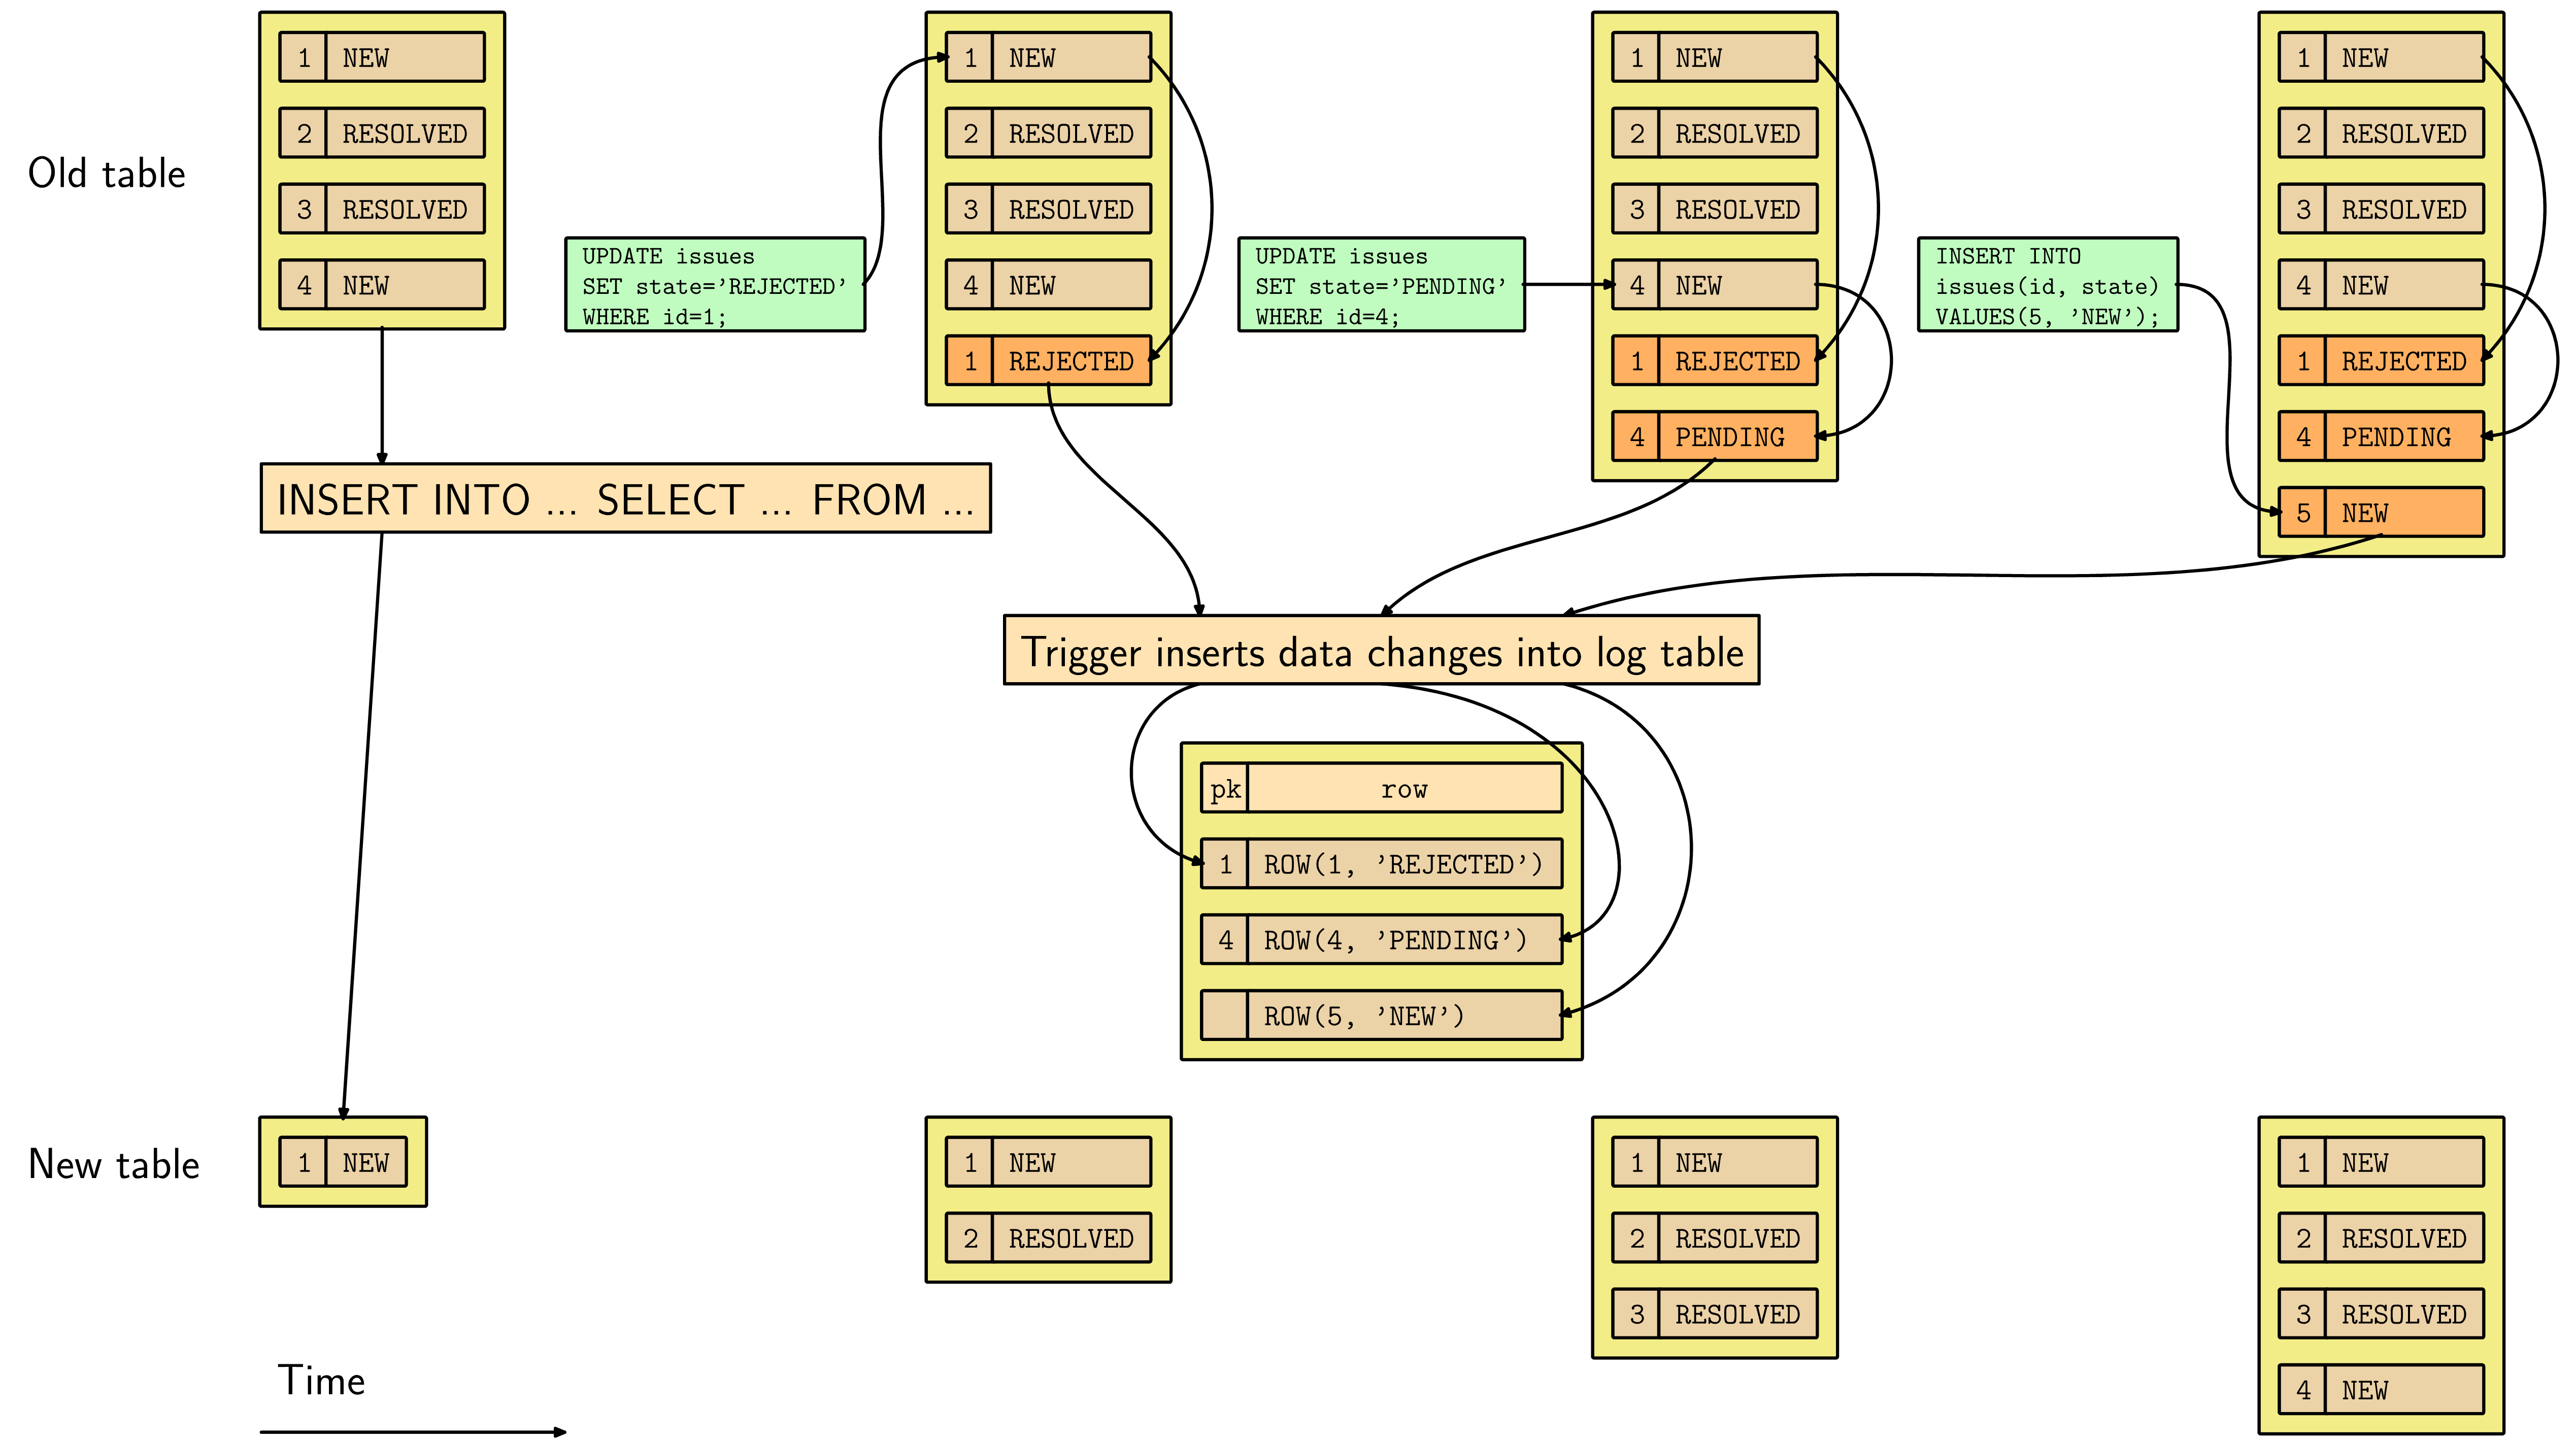
\includegraphics[height=\sizeforimages\textheight]{images/pg_repack_01.png}
  \end{center}
\end{frame}

\begin{frame}
  \frametitle{\texttt{pg\_repack}}
  \begin{center}
    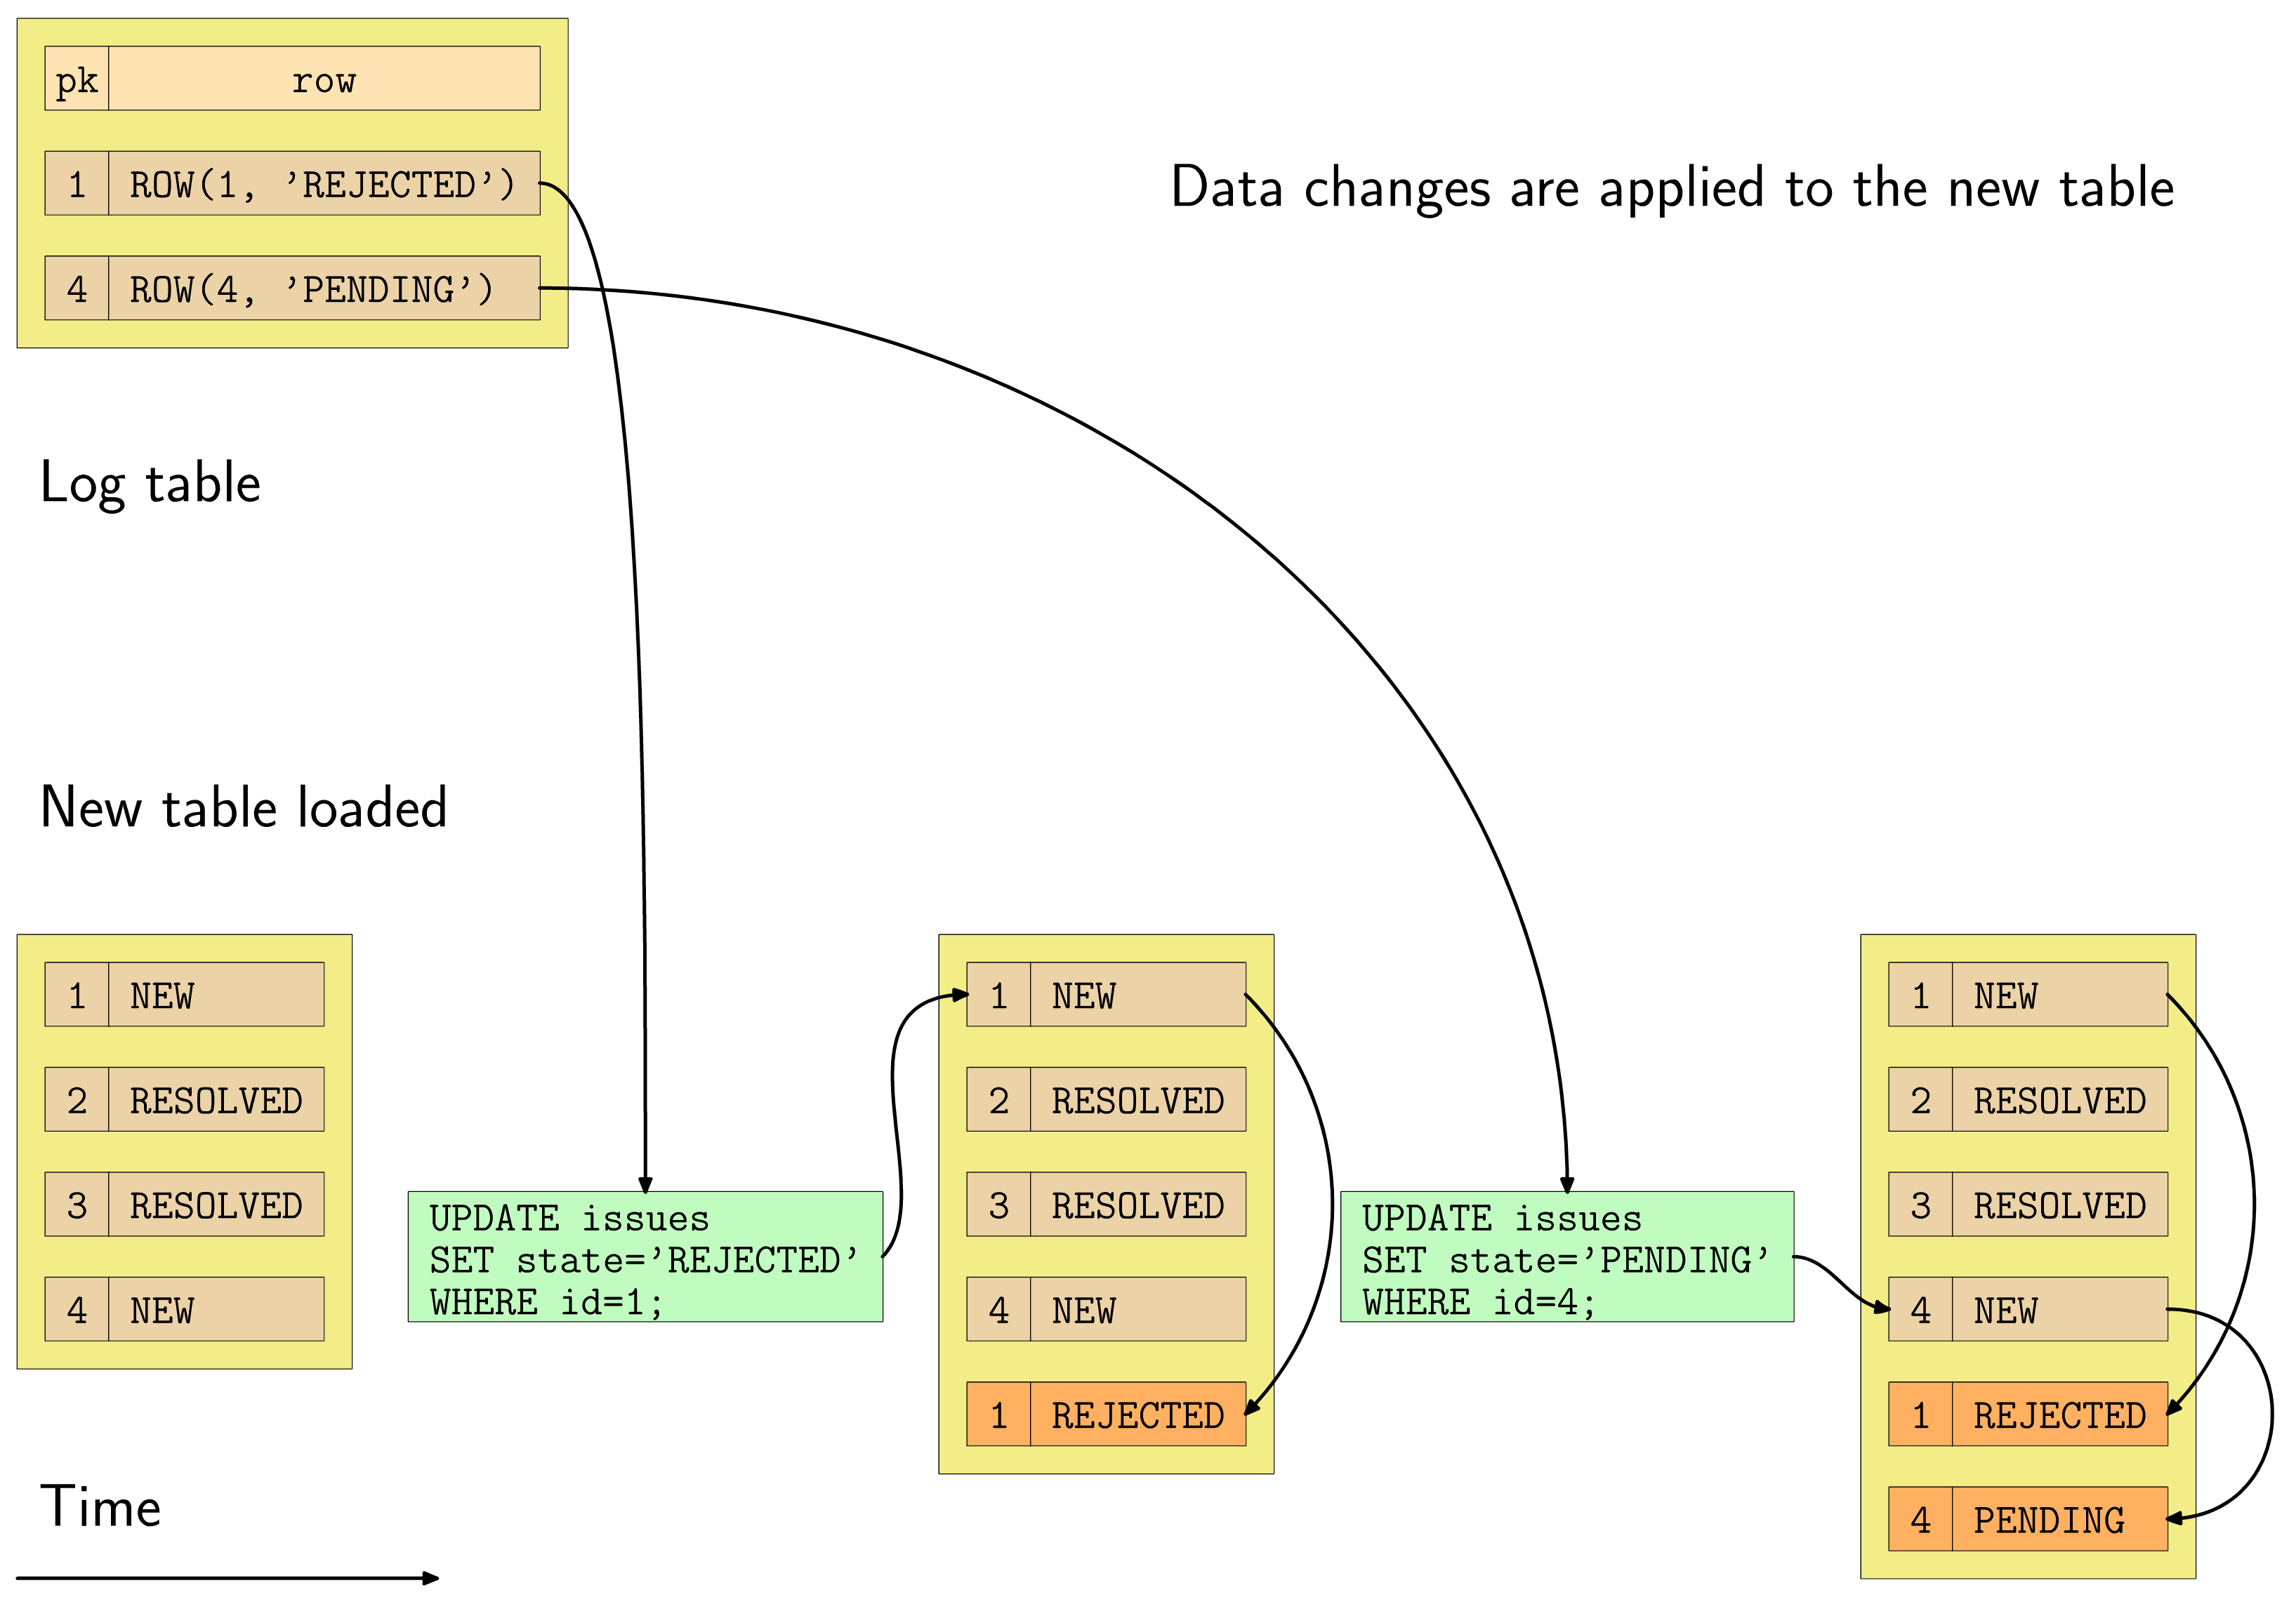
\includegraphics[height=\sizeforimages\textheight]{images/pg_repack_02.png}
  \end{center}
\end{frame}

\begin{frame}
  \frametitle{\texttt{pg\_repack}'s algorithm}
  \begin{itemize}
    \item Like \texttt{VACUUM FULL}, it removes bloat by copying the
      useful data to a new table, swaps underlying files and drops the new
      table.
    \item Exclusive lock is held during the swap, but possibly a bit longer if
      the database is very busy.
    \item Data changes done by applications during the copy are captured by
      triggers and written to a ``log table'';
      applied after the initial copying and index rebuild, right before the swap.
    \item Multiple backends can be launched to rebuild indexes
  \end{itemize}
\end{frame}

\begin{frame}
  \frametitle{\texttt{pg\_squeeze}}
  \begin{itemize}
    \item Started in 2016 (PostgreSQL 9.5)
    \item Initial motivation: allow \texttt{pg\_repack} to be scheduled without external tools
    \item Use of dual client/server implementation made this difficult
    \item Realization: better to reimplement everything with modern technology
      \begin{itemize}
	  \relscale{0.8}
	\item background worker for scheduling (requires server-only code)
	\item logical decoding (instead of triggers)
        \item binary data rather than text
        \item server API rather than SQL commands
      \end{itemize}
    %% This might not be wrong but it does not fit on the page.
    \item End result: a complete reimplementation
  \end{itemize}
\end{frame}

\begin{frame}
  \frametitle{\texttt{pg\_squeeze}}
  \begin{center}
    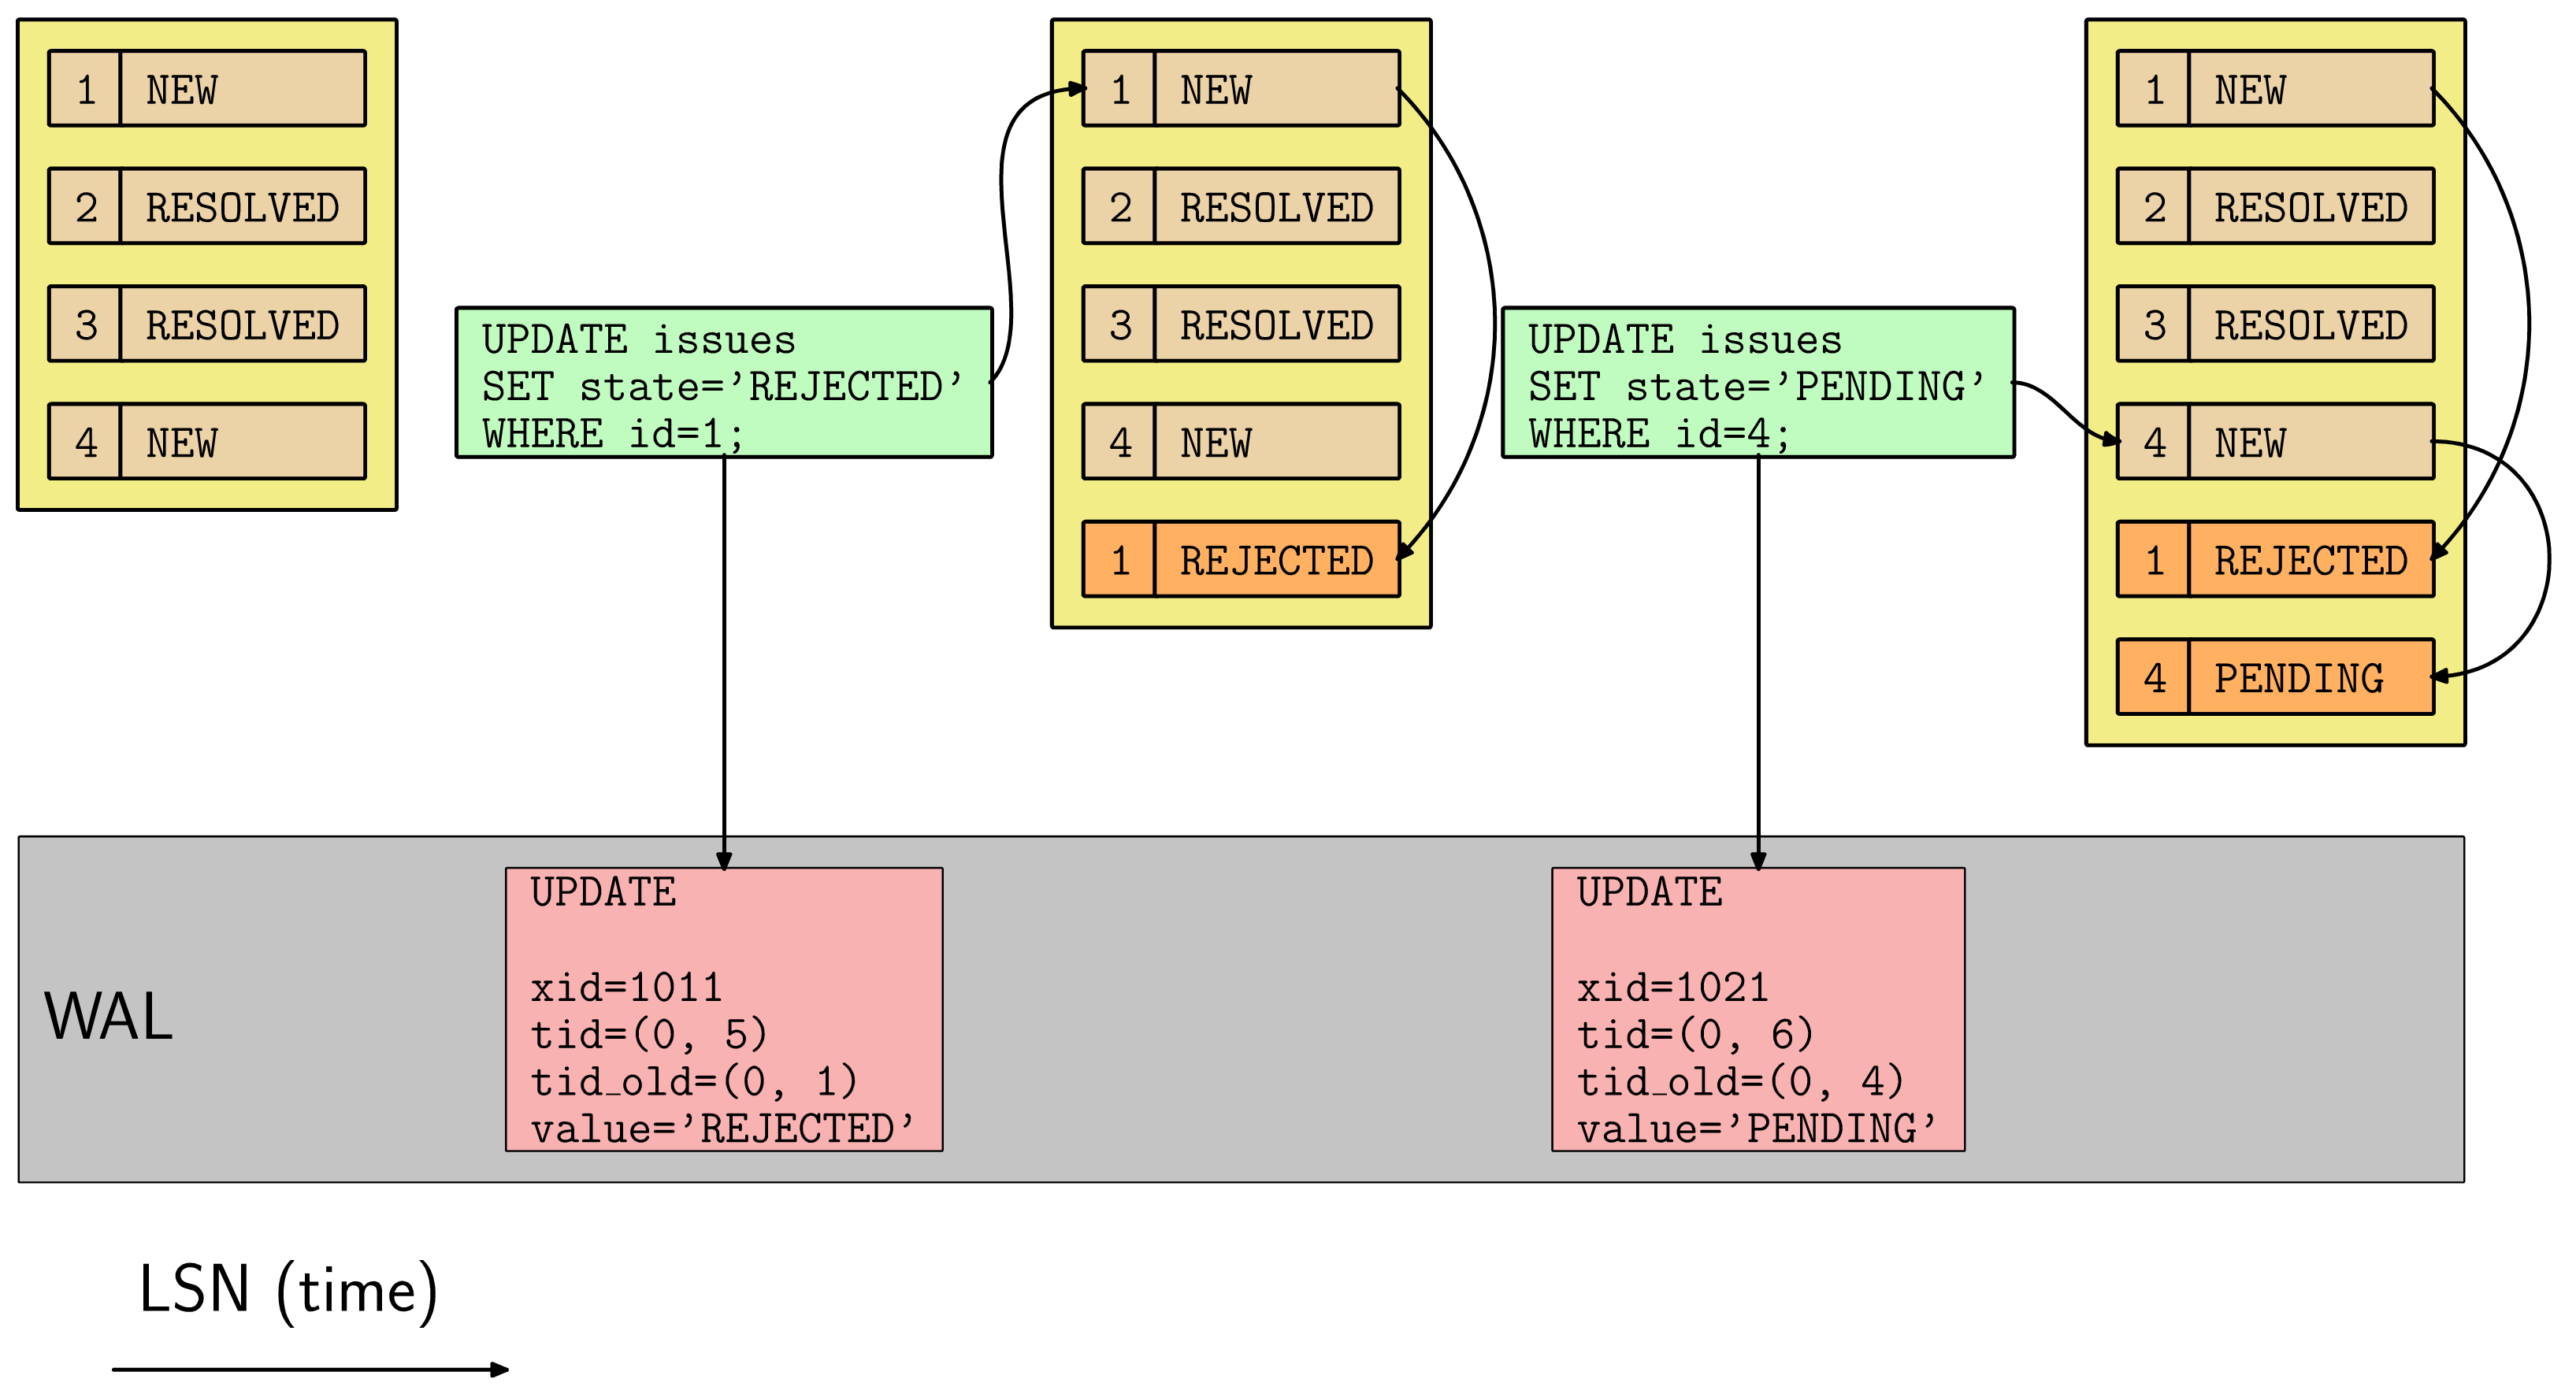
\includegraphics[height=\sizeforimages\textheight]{images/pg_squeeze_01.png}
  \end{center}
\end{frame}

\begin{frame}
  \frametitle{\texttt{pg\_squeeze}}
  \begin{center}
    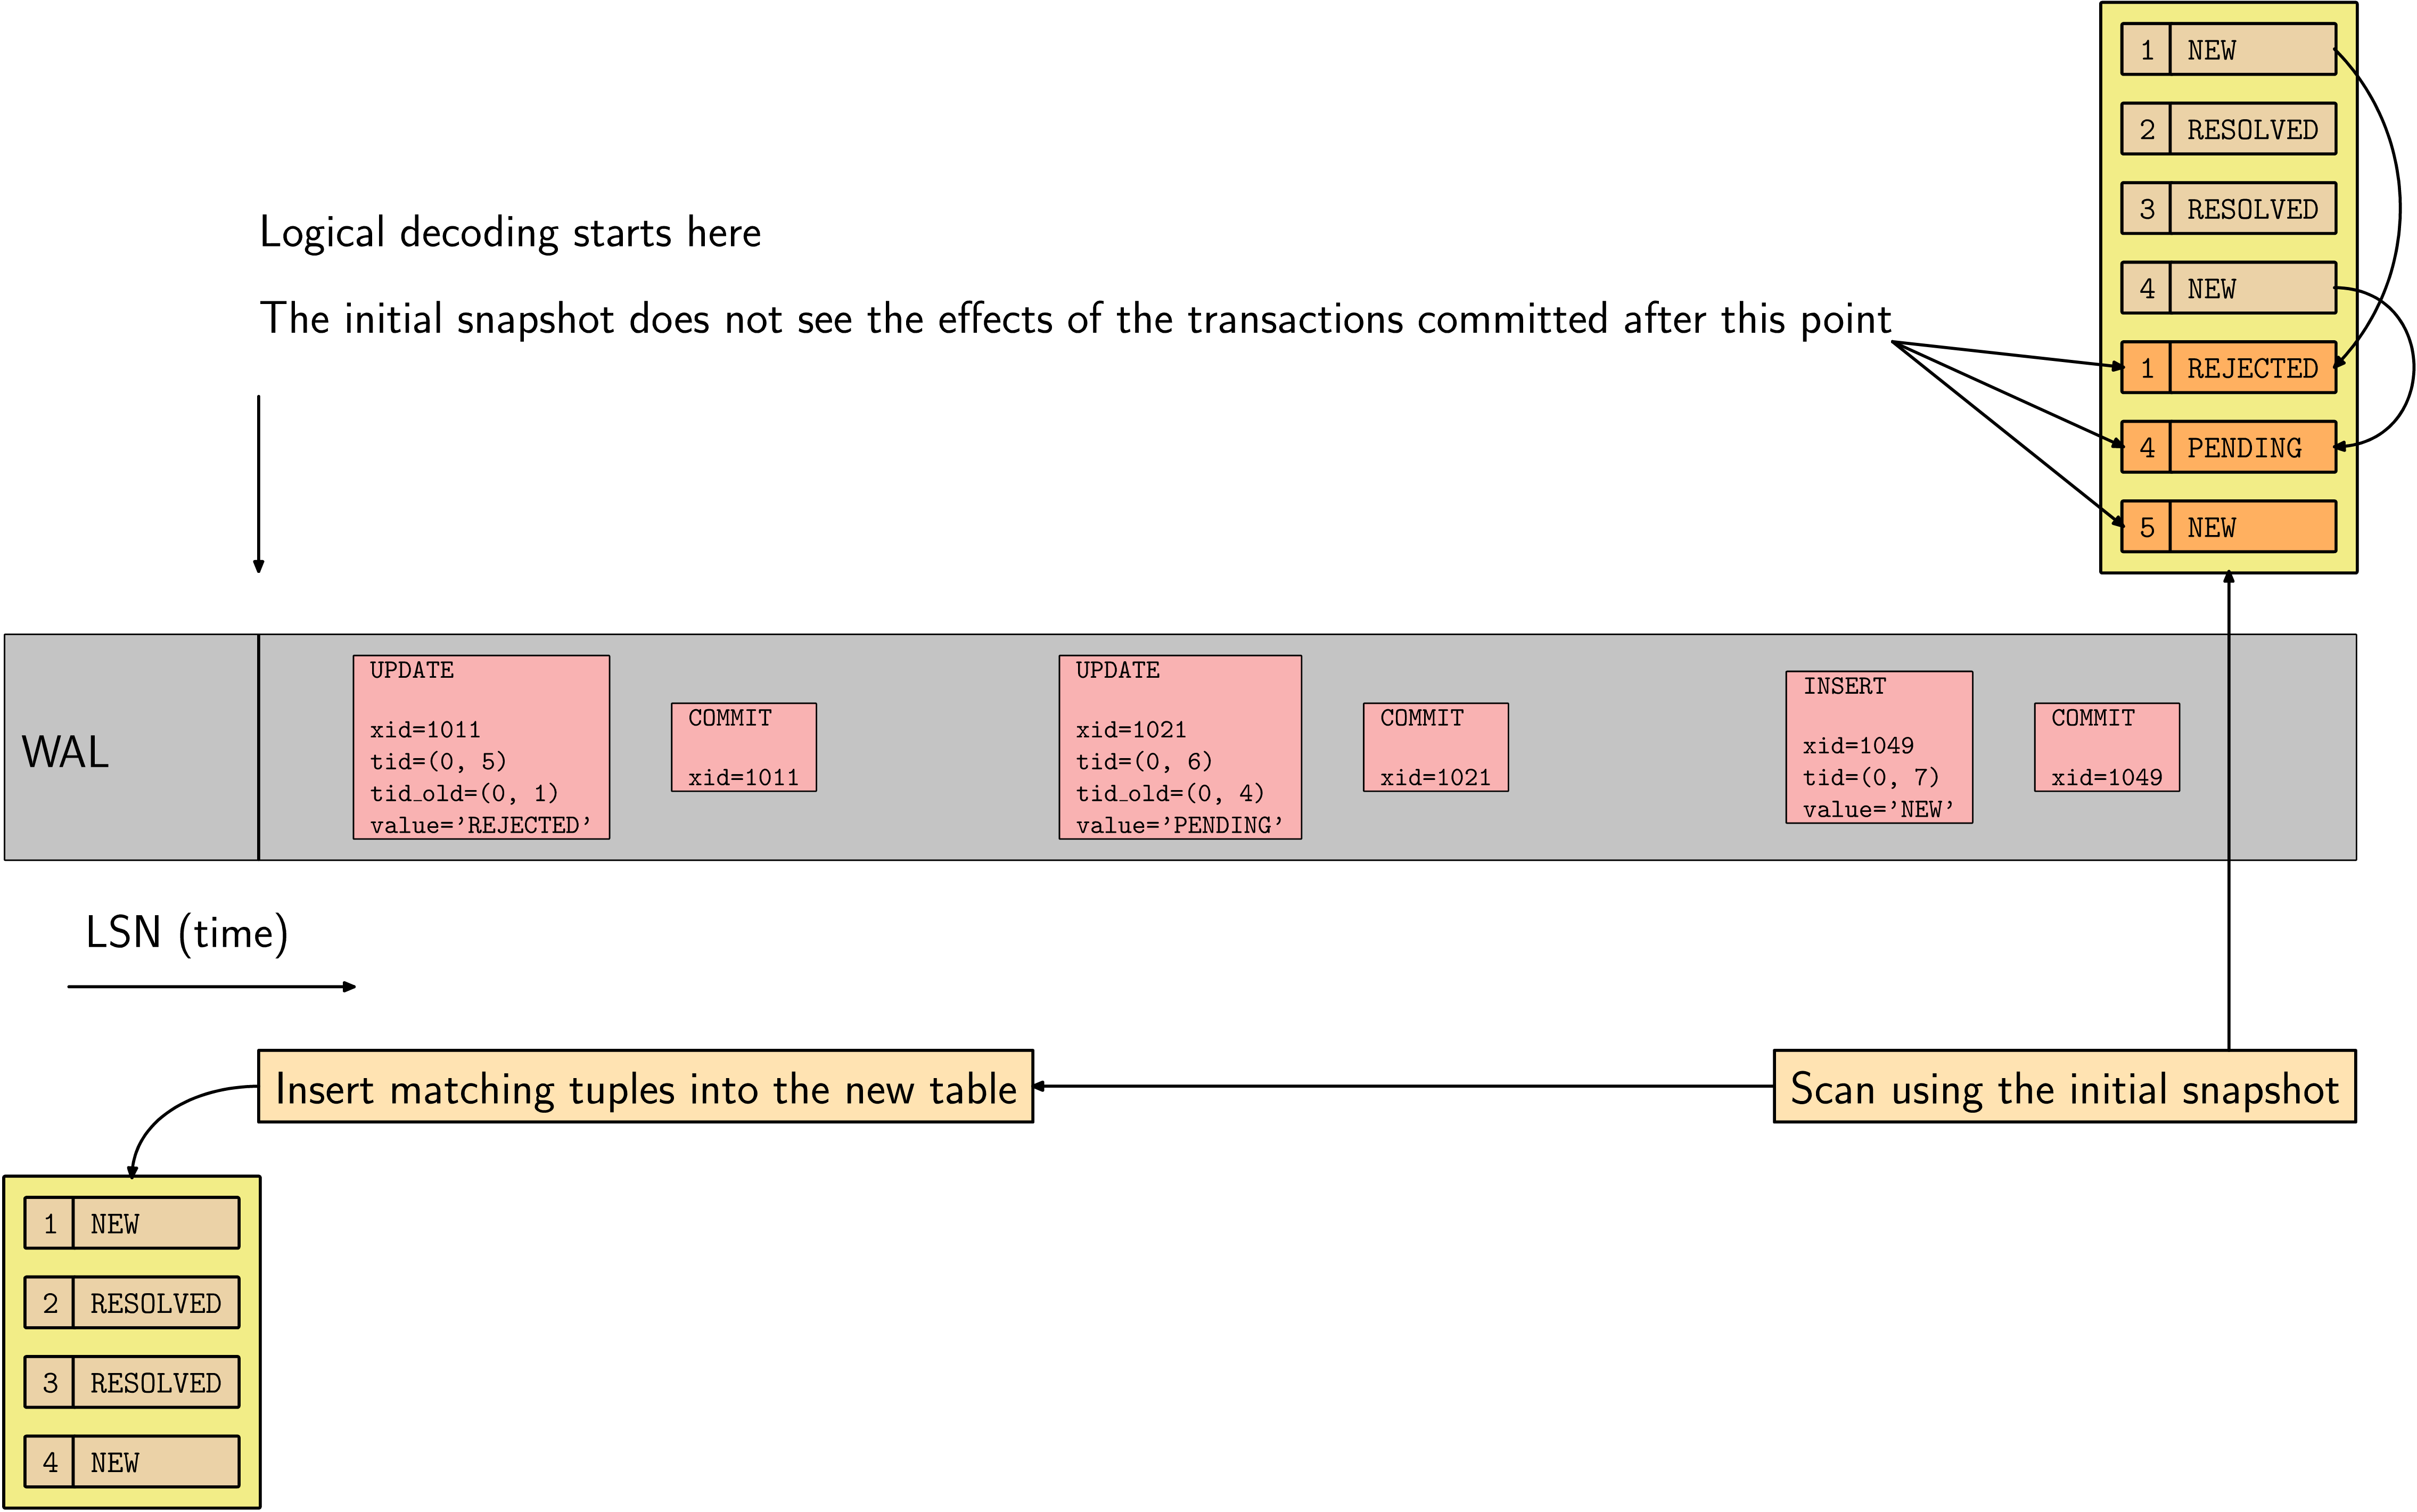
\includegraphics[height=\sizeforimages\textheight]{images/pg_squeeze_02.png}
  \end{center}
\end{frame}

\begin{frame}
  \frametitle{\texttt{pg\_squeeze}}
  \begin{center}
    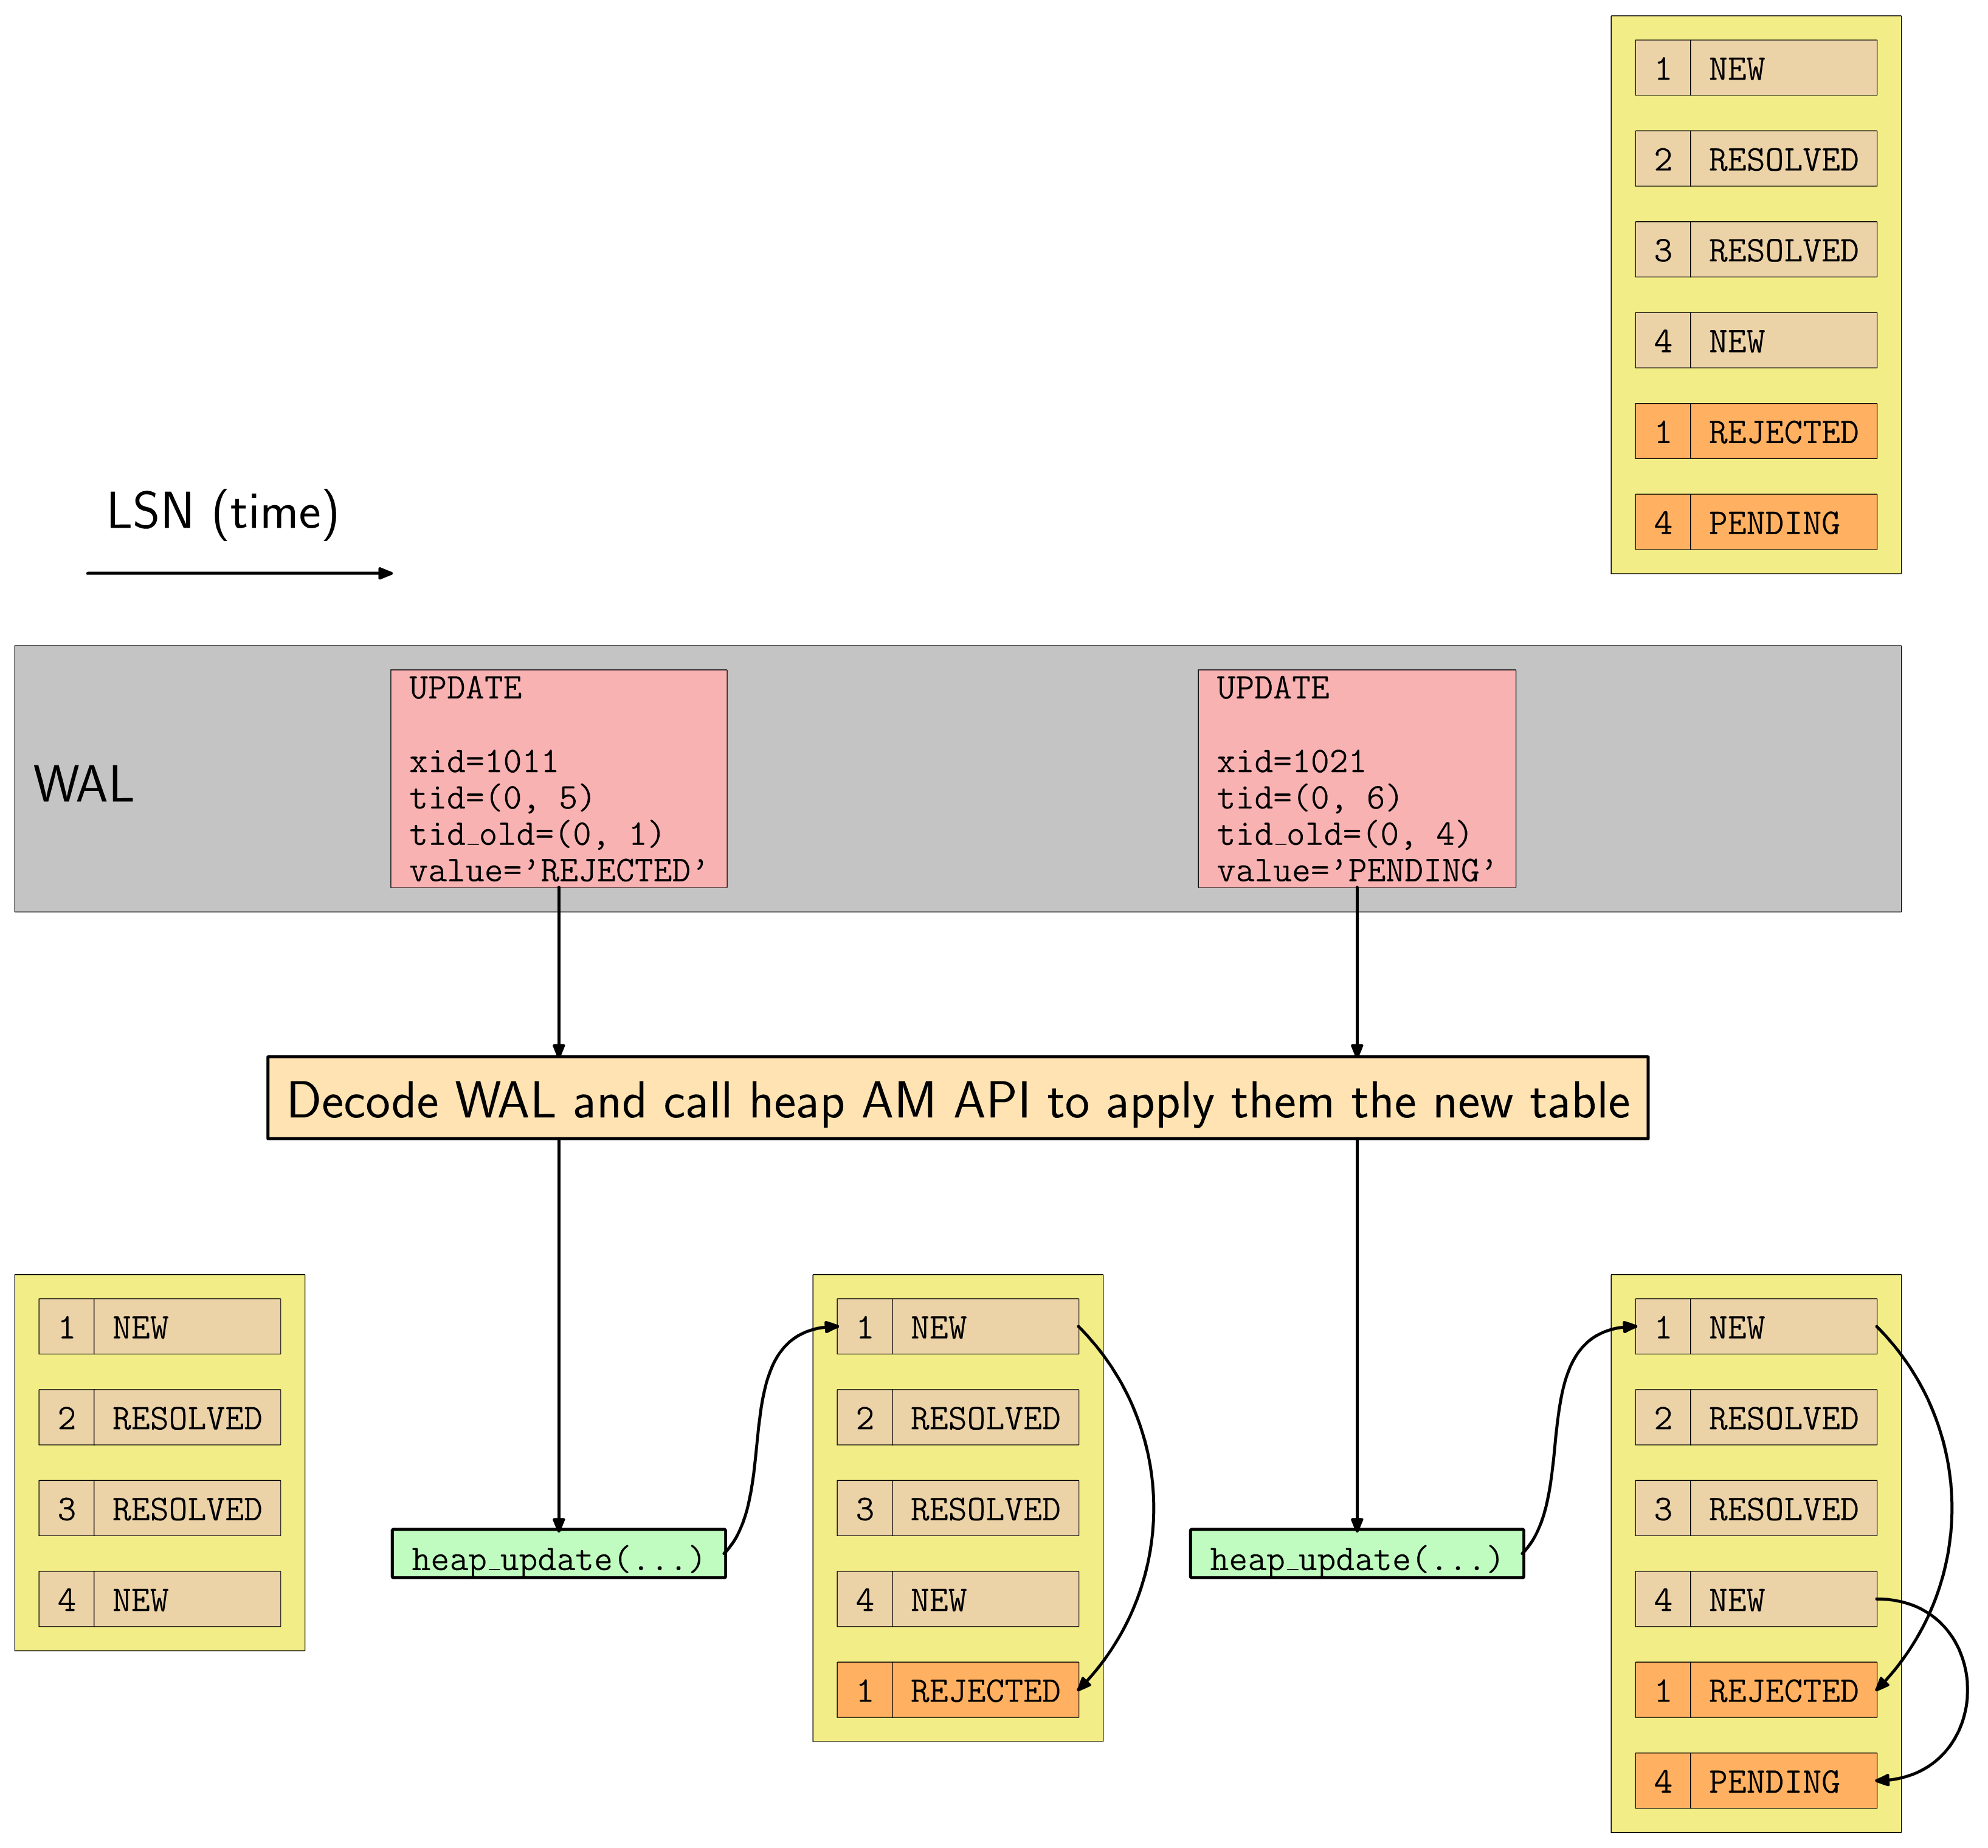
\includegraphics[height=\sizeforimages\textheight]{images/pg_squeeze_03.png}
  \end{center}
\end{frame}

\begin{frame}
  \frametitle{\texttt{pg\_squeeze}}
  \begin{itemize}
    \item cron-like scheduling. Squeeze table if the portion of bloat exceeded
      threshold specified by the DBA.
  \end{itemize}
\end{frame}

%% TODO 1. Disk space requirements, 2. GUC for maximum lock time (probably not
%% used much)
%% \begin{frame}
%%         \frametitle{\texttt{pg\_squeeze}}
%\end{frame}

\begin{frame}
  \frametitle{The REPACK command}
  \begin{itemize}
    \item \texttt{REPACK} subsumes \texttt{CLUSTER} and \texttt{VACUUM FULL}
  \end{itemize}
  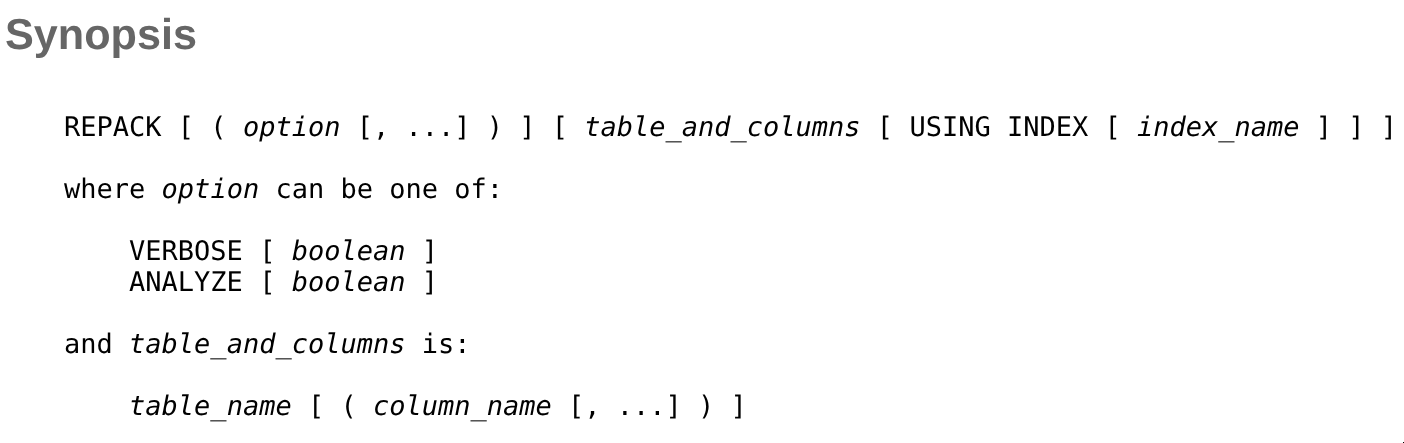
\includegraphics[width=\textwidth]{repack.png}
\end{frame}

\begin{frame}[fragile]
  \frametitle{Single-table \texttt{REPACK} forms}
  \begin{itemize}
    \item single-table \texttt{vacuum full}:
      \begin{lstlisting}
REPACK (ANALYZE) customers;
      \end{lstlisting}
    \item single-table \texttt{cluster}:
      \begin{lstlisting}
REPACK (ANALYZE, VERBOSE) customers USING INDEX cust_pkey;
      \end{lstlisting}
    \item single-table \texttt{cluster} using the stored index:
      \begin{lstlisting}
REPACK customers USING INDEX;
      \end{lstlisting}
  \end{itemize}
\end{frame}

\begin{frame}[fragile]
  \frametitle{Full-database \texttt{REPACK} forms}
  \begin{itemize}
    \item whole-database \texttt{VACUUM FULL}:
      \begin{lstlisting}
REPACK;
      \end{lstlisting}
    \item whole-database \texttt{CLUSTER}:
      \begin{lstlisting}
REPACK USING INDEX;
      \end{lstlisting}
  \end{itemize}
\end{frame}

\begin{frame}[fragile]
  \frametitle{Concurrent \texttt{REPACK}}
  \begin{lstlisting}
REPACK (ANALYZE, CONCURRENTLY) customers USING INDEX tenant_idx;

REPACK (CONCURRENTLY) orders;

REPACK (CONCURRENTLY) USING INDEX;
  \end{lstlisting}
  \begin{itemize}
    \item This behaves similar to \texttt{pg\_squeeze}
    \item Differences of note:
      \begin{itemize}
	\item Does not unlock the table before requesting the exclusive lock.
	\item No scheduling -- do we need that in core?
      \end{itemize}
  \end{itemize}
\end{frame}

\begin{frame}
  \frametitle{Concurrent REPACK (2)}

  Advantages over \texttt{pg\_squeeze}:

  \begin{itemize}
      % This is not yet implemented I think, so let's mention it in
      % "Future work"
%    \item Should not require {\tt wal\_level=logical}
    \item Should not restrict VACUUM of other tables (problem of ``xmin
      horizon``)
    \item MVCC safety (hopefully in PG 19)
    \item Fully integrated in core
    \begin{itemize} \item Very easy to use \end{itemize}
  \end{itemize}

\end{frame}

% TODO (if there's enough time) Explain differences between pg_squeeze and
% REPACK CONCURRENTLY.
%
% 1. pg_squeeze uses AccessShareLock and releases it before it requests
% AccessExclusiveLock (for the file swap), in order to avoid deadlock. If the
% table changed in between, the whole processing is aborted. This approach is
% proably overly cautious. In REPACK CONCURRENTLY, we use
% ShareUpdateExclusiveLock and then simply upgrade it to AccessExclusiveLock,
% so we don't have to check for concurrent catalog changes. (The risk of
% deadlock during the lock upgrade is probably low.)
%
% 2. Since REPACK CONCURRENTLY does not release the ShareUpdateExclusiveLock
% until done, and since this lock conflicts with VACUUM, it does not have to
% care about the xmin horizon (Note: setting the slot's xmin to
% InvalidTransactionId is yet to be implemented.) On the other hand,
% pg_squeeze allows for VACUUM most of the time, so has to block the xmin
% horizon until the initial copy is complete.
%
% 2. Unlike extension, the core code can implement MVCC safety. (Although not
% necessarily in PG 19).
%
% 3. REPACK does not implement scheduling - not sure it's necessary,
% extensions can do that.
\end{frame}

\begin{frame}
  \frametitle{\texttt{pg\_repackdb}}

    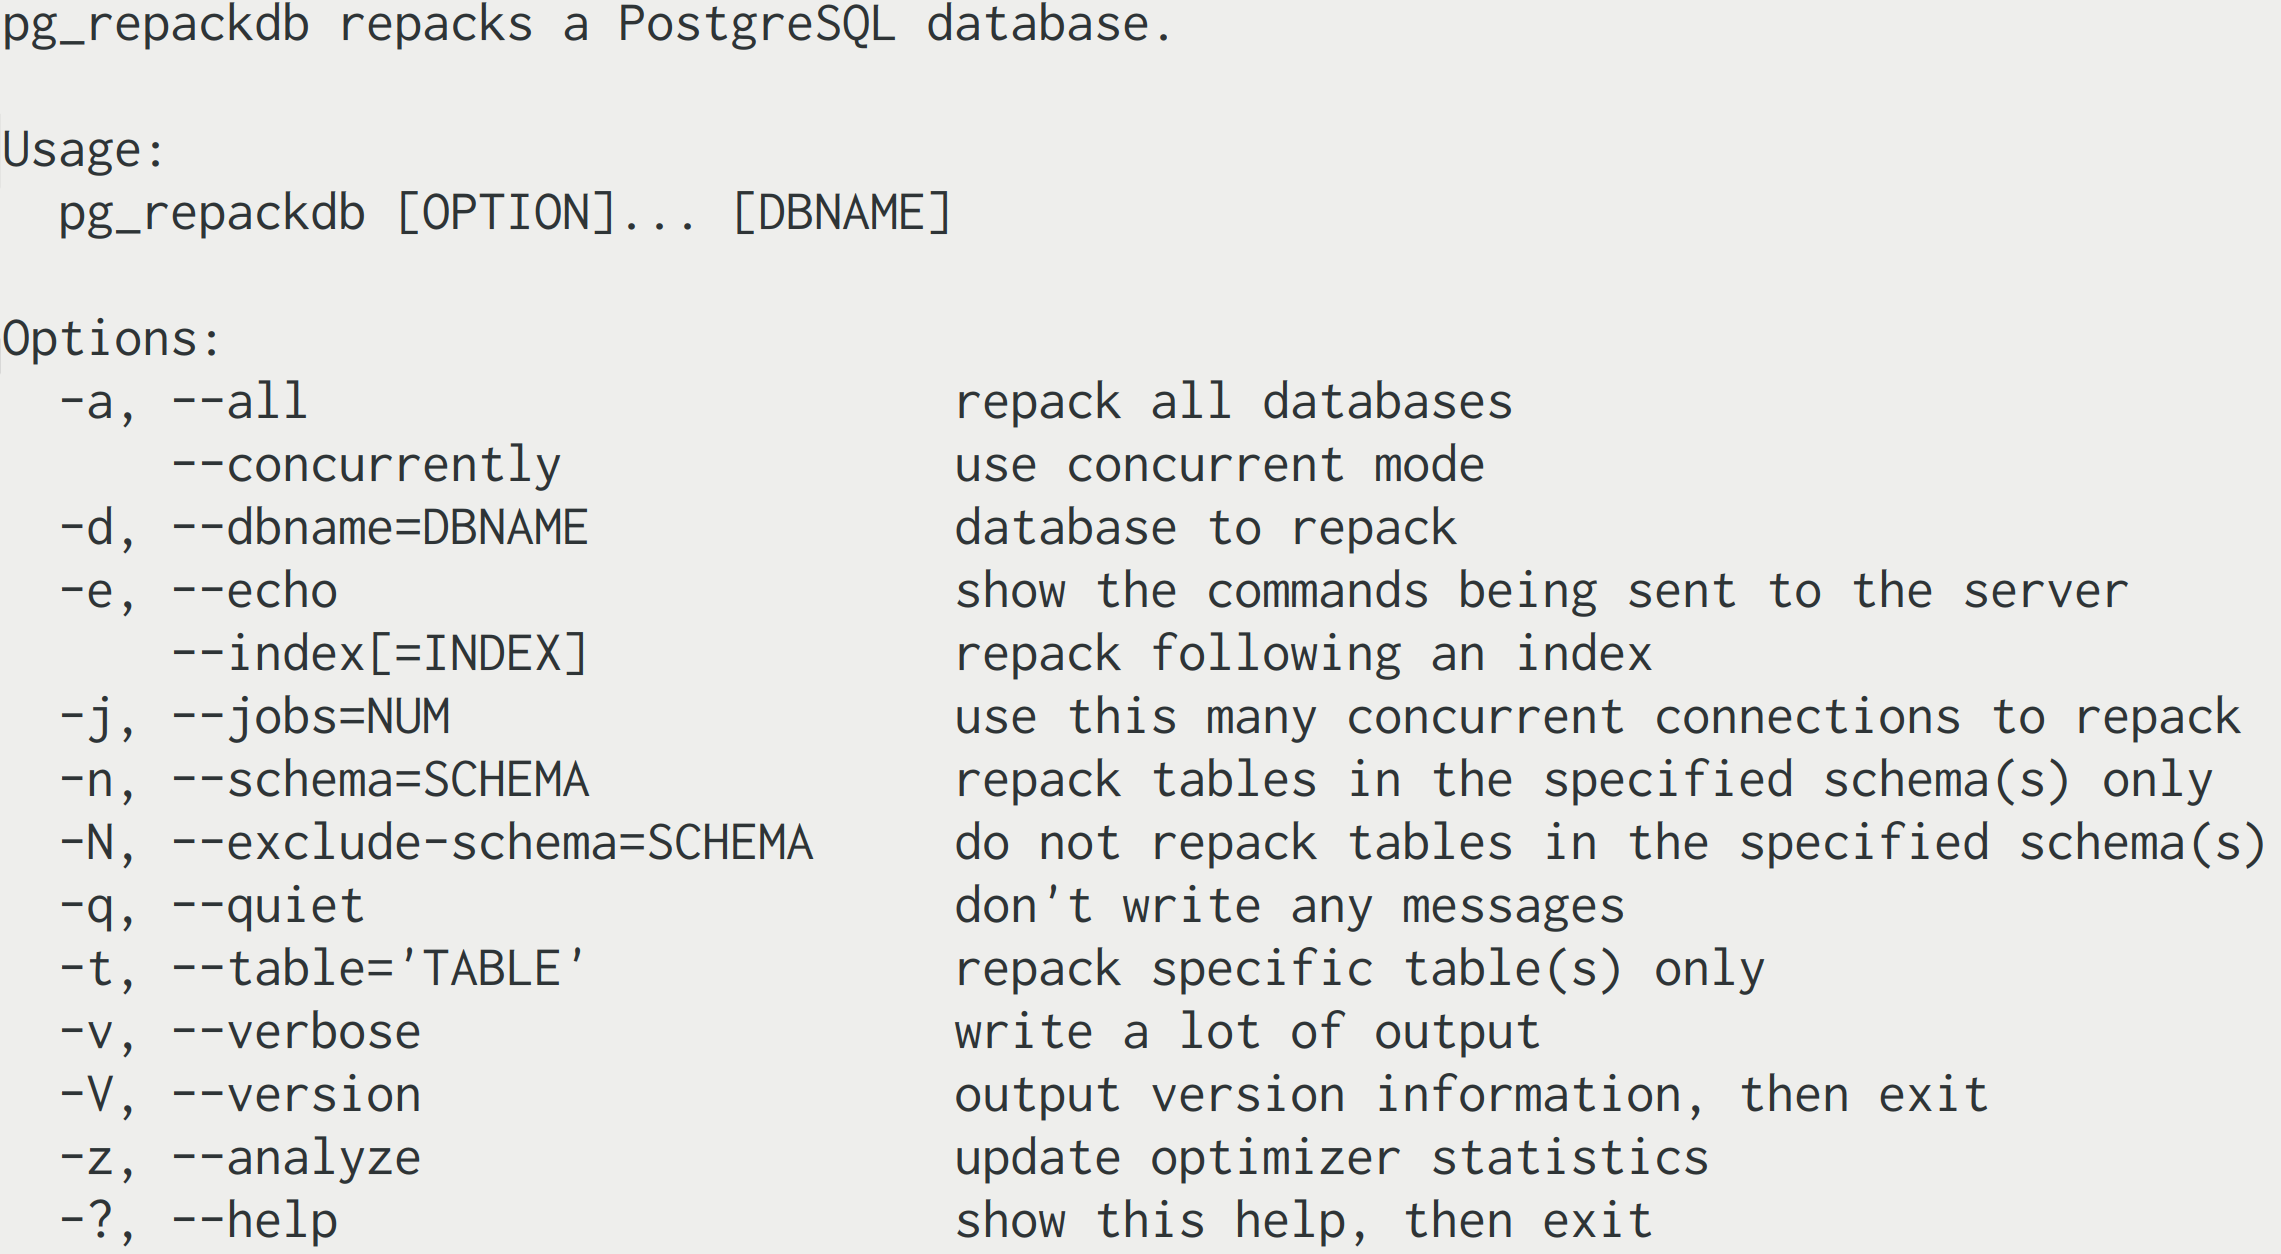
\includegraphics[height=\sizeforimages\textheight]{repackdb.png}
\end{frame}

\begin{frame}
  \frametitle{Future work}
  \begin{itemize}
    \item allow to enable logical decoding on the fly
    \item use a background worker for logical decoding
    \item Better control over repacking multiple tables
  \end{itemize}
\end{frame}

\begin{frame}
  \frametitle{Call to Action!}

  \begin{itemize}
    \item First things first: do you like \texttt{REPACK}?
    \item Test the patch! \href{https://commitfest.postgresql.org/patch/5117/}{https://commitfest.postgresql.org/patch/5117/}
  \end{itemize}
\end{frame}
